%Chapter 3: Rapid Static Modeling

\chapter{Rapid Static Modeling}

In the introductory chapter we discussed how recent response to large earthquakes has been limited by a strict reliance on seismic data for early characterization of the earthquake source. In Chapter 2 we discussed briefly the problems facing traditional seismological instrumentation at local and regional distances of large events. Seismometers clip during strong shaking and strong motion sensors are beleaguered by baseline offsets. The latter problem, baseline offsets, is particularly important because it affects the long period band of seismic time series. it is precisely this frequency band that is most useful for discerning the broad features of large earthquakes. If a geophysical instrument is band limited then it will become increasingly difficult to differentiate between say a magnitude 7 and a magnitude 8 event. This is a condition known as saturation and it is common in early warning algorithms that rely on seismometers and accelerometers alone \cite{Brown2011}.

Large events induce a permanent deformation of the Earth's crust, the static field. If the earthquake is large enough, and the geophysical sensor close enough or sensitive enough it is possible to measure the static field. For hazards applications this is of great interest because the static field is a zero frequency wave and as such the longest period information we can measure about an event. Thus characterization of the static field and of its contribution to a seismogram solves the problem of saturation. Furthermore the static field can be to first order assumed to have no time dependence, this makes it simple to extend earthquake source models from point sources to more realistic and complex geometries without consideration for the time-dependent effects of linear superposition.

Although noisier than accelerometers, GPS can easily record the permanent deformation at regional distances of large earthquakes, this was documented as far back as the 1992 M7.2 Landers earthquak \citep{bock1993,blewitt1993}.  It has since become routine to observe coseismic offsets in post-processed GPS time series after medium to large events and discussion in the literature of the potential of static field modeling for rapid response has become vigorous. \citet{Blewitt2006} showed that given an epicentral location and assuming thrust faulting for the 2004 Mw 9.2  Sumatra-Andaman earthquake, one could have estimated an accurate magnitude within 15 minutes of the origin time using global GPS stations at regional to teleseismic distances. \citet{sobolev2007} proposed and demonstrated the viability of a system that uses coseismic offsets from GPS to directly invert for a heterogeneous slip model. \citet{Crowell2012} produced heterogeneous coseismic slip inversions from real-time data for two large events and \citet{Wright2012} produced source models with 4 fault patches from precise point positioning data for the M9 Tohoku-oki earthquake. \citet{Ohta2012} were able to produce in simulated real-time mode a simple uniform slip source model for the 2011 Tohoku-oki event and discussed the viability of using such a model to simulate tsunami propagation. \citet{PerezCampos2013} computed similar models for one scenario and one recorded subduction event in Mexico with a sparse network. This patchwork of studies demonstrate to varying degrees the viability, interest and importance of rapid modeling algorithms that employ the static field.

Throughout this chapter we will discuss a coherent framework that demonstrates how such recordings can be used. We will demonstrate the logical progression from point source centroid moment tensor models to finite extent moment tensors and finally slip inversions.

The Kalman filter method discussed in the previous chapter aides these algorithms insofar as it allows for better quantification of static offsets by reducing the noise in the displacement time series. Most notably there can be an order or more magnitude improvement in the resolution of vertical offsets. Nonetheless, its net effect, while non-negligible, is not of paramount importance for point source and finite extent moment tensor computation. These methods can be quite successful with GPS data alone. The along-dip resolution in slip inversions does improve with seismogeodetic estimates of the static field, although again, it can still be adequately computed with GPS data alone. Later on in Chapter 4 we will see the true benefit of the filtered data for source estimation when we compute kinematic models.

\section{Centroid Moment Tensor Inversion}
\label{sec:cmt}

Computation of the seismic moment tensor (MT) for a given earthquake is one of the fundamental kinds of modeling performed to study the source. The moment tensor can be calculated from a number of methods such as polarity of first arrivals \citep{Havskov2010} or waveform matching \citep{dreger2003} and is a compact representation of the source that contains basic information on the size of the event, the fault plane geometry and the style of faulting. Moment tensor solutions are of use over a range of earthquake magnitudes. Small to medium events are utilized for tectonic studies and to determine the stress regime within a region. For large events, rapid determination of the centroid location as well as the moment tensor (CMT) provides valuable information for earthquake response, tsunami early warning and as a starting point for finite fault source modeling.

Currently there are a number of efforts that routinely compute moment tensor solutions for earthquakes worldwide. The most comprehensive catalogue of such solutions is contained in the Global Centroid Moment Tensor (GCMT) Project. At its inception the GCMT project included inversion of body and surface waves \citep{dziewonski1981,dziewonski1983} and has seen numerous refinements since such as inclusion of aspherical Earth structure, attenuation, etc. This method however employs only teleseismic data and its emphasis is in data collection and catalogue compilation not in rapid modeling. Real-time moment tensors can be obtained for small to medium events using time domain waveform matching inversion schemes  \citep{dreger1990,dreger1993}. However, real-time CMT determination of medium to large events is still an active area of research.

One of the most important advances in computing CMTs as quickly as possible for large events is contained in the work of \citet{kanamori2008} who elaborated on \citet{kanamori1993}'s observation of the W phase, a long period phase arriving in between the direct P and S waves. They showed that inversion for the moment tensor using data as close as 15$^\circ$ from the source is viable. W phase inversion algorithms currently run in real time at the USGS, Pacific Tsunami Warning Center (PTWC) and Institut du Physique du Globe de Strasbourg (IPGP-EOST) \citep{hayes2009}. Since the W phase arrives well before large amplitude surface waves and remains on-scale far longer such inversion algorithms have shown to be a marked improvement in rapid computation of moment tensor solutions for large events over traditional waveform matching techniques. 

Following the Mw 9.0 Tohoku-oki earthquake, \citet{duputel2011} showed that it was feasible to use data at distances as small as 11$^\circ$ from the source. However, W phase based inversion schemes, while very robust, require long period displacement records (e.g. 200-1000s for the 2011 Tohoku-oki event) \citep{duputel2011}. Such recordings, as discussed before, are almost always unusable close to the source in real time; velocity instruments clip and it is difficult to extract long period motions from strong-motion accelerometer data in real time.

Thus, there seems to be a limitation in how fast moment tensor solutions can be obtained operationally for large events using seismic instruments and existing seismological methods. For example, for the Tohoku-oki event it took 20 minutes after origin time to arrive at the first CMT solutions by agencies running W phase algorithms \citep{duputel2011}, even though the rupture had a duration of three minutes \citep{simons2011}. This delay was due to the reliance on teleseismic data. After several iterations using progressively more data, the final CMT solution \citep{hayes2011} was obtained 90 minutes after origin time using data up to 90$^\circ$ from the rupture. The first estimate of moment magnitude was obtained in about 3 minutes by the Japan Meteorological Agency (JMA), but was grossly underestimated at Mw 6.8. \citet{duputel2011} documented that in the numerous iterations between agencies the nodal planes were somewhat consistent with only minor variations in strike dip and rake, the magnitudes oscillated between Mw 8.8-9.0 after the 20-minute mark, but the centroid locations varied by as much as 2$^\circ$ and 60km in depth. 


\subsection{Point Source Models}

We present a robust method for determining CMT solutions that is considerably faster than current seismic methods, based on real-time high-rate displacement data from near-source GPS stations. Although we are not explicitly solving for the style and geometry of faulting, that information is implicit in the moment tensor solution. In general, we do not require prior knowledge of the sense or extent of faulting, although that information could be used if available.
We demonstrate the new algorithm by replaying the estimation of 1Hz displacements for the 2003 Mw 8.3 Tokachi-oki earthquake using GPS data from Japan�s GPS network (GEONET) \citep{Miyazaki1998} and for the 2010 Mw 7.2 El Mayor-Cucapah earthquake using data from the California Real Time Network (CRTN) \citep{Bock2004}. We will also discuss the limitations of the point source strategy as  illustrated by the Mw 9.0 Tohoku-oki earthquake.

\subsubsection{Extracting Coseismic Offsets}

Our inversion schemes use coseismic offsets, we apply a 120s moving average filter to the 1Hz displacement waveforms to remove the dynamic component and retain the information on the permanent deformation. GPS data have much higher noise levels than traditional seismological data sets in particular in the vertical direction, thus, we set a threshold of 15mm on the total horizontal component at a given station. This is roughly 3 times the usual noise level in the horizontal component of real-time GPS measurements \citep{genrich2006}.  At any given epoch only stations over this threshold are considered for the inversion.

\subsubsection{Inversion Scheme}

The inversion scheme employed here relates the coseismic offset measured at the surface to source parameters at depth. \citet{Amoruso2004} and \citet{Hearn2005} showed that crustal layering can have a significant effect when inverting for source parameters using static offsets, thus we must account for, at least, a simple one-dimensional structure. To do so we compute Green's functions (GFs) using Fortran codes EDGRN/EDCMP \citep{wang2003} for a 1D layered Earth. This numerical approach starts from the closed form solutions of the partial differential equations of motion obtained from the Hankel transform and then applies a Thomson-Haskell propagator matrix to relate the deformation at depth with that at the surface. We extract the GFs from the code output and set up the kernel matrix $\mathbf{G}$ for the inversion :
\begin{equation}
\left(\begin{matrix}
 u_1^1\\
 u_2^1\\
 u_3^1\\
 \vdots\\
 u_1^n\\
 u_2^n\\
 u_3^n\\
\end{matrix}\right)
=
\left(\begin{matrix}
G^1_{11} & G^1_{12} & G^1_{13} & G^1_{14} & G^1_{15}\\
G^1_{21} & G^1_{22} & G^1_{23} & G^1_{24} & G^1_{25}\\ 
G^1_{31} & G^1_{32} & G^1_{33} & G^1_{34} & G^1_{35}\\
\vdots &  & \cdots &  & \vdots\\
G^2_{11} & G^2_{12} & G^2_{13} & G^2_{14} & G^2_{15}\\
G^2_{21} & G^2_{22} & G^2_{23} & G^2_{24} & G^2_{25}\\ 
G^2_{31} & G^2_{32} & G^2_{33} & G^2_{34} & G^2_{35}\\
\end{matrix}\right)
\left(\begin{matrix}
 m_1\\
 m_2\\
 m_3\\
 m_4\\
 m_5\\
\end{matrix}\right)\;,
\end{equation}
or more succinctly
\begin{equation}
\label{eq_mshort}
u_i^k=G^k_{ij}m_j\;;\;\{i=x,y,z\;,\;j=1,2,\dots,5\;,\;k=1,2,\dots,n\}\;,
\end{equation}
where $u_i^k$ is the $i$-th component of displacement measured at the $k$-th station, $m_j$ is the $j$-th component of the moment tensor and $G_{ij}^k$ are the $i$-th component GFs that relate the $j$-th component of the moment tensor to the $k$-th station. Thus the GF matrix is very compact, having only 5 elements per direction of motion per station.

The moment tensor in this case is composed of 5 components since we restrict the inversion to the deviatoric portion such that for the general six component symmetric Cartesian MT
\begin{equation}
\label{eq_mcart}
\mathbf{M}
=
\left(\begin{matrix}
m_{xx} & m_{xy} & m_{xz}\\
m_{xy} & m_{yy} & m_{yz}\\
m_{xz} & m_{yz} & m_{zz}\\
\end{matrix}\right)\;,
\end{equation}
the deviatoric restriction means that the following equivalences between Equations \ref{eq_mshort} and \ref{eq_mcart} hold
\begin{eqnarray}
m_1&=&m_{xy}\nonumber\\
m_2&=&m_{xz}\nonumber\\
m_3&=&m_{zz}\nonumber\\
m_4&=&(1/2)(m_{xx}-m_{yy})\nonumber\\
m_5&=&m_{yz}\;.
\end{eqnarray}
We have retained the \citet{Aki2002} convention where $x$ is north, $y$ is east and $z$ is down. This is just one of many possible moment tensor coordinate representations; however we have chosen this one to be consistent with the notation used by the EDGRN/EDCMP software.

Since we are making a point source approximation and neglecting fault finiteness, we assume that despite the coseismic motions the source to receiver distances remain unchanged and so the Green�s function matrix remains unaltered throughout the inversion process. Next we assemble the data vector from that epoch�s measured coseismic offset and weigh the data by the pre-event standard deviations as
\begin{equation}
\textbf{Wu}=\textbf{WGm}\;,
\end{equation}
where
\begin{equation}
\textbf{W}=\mathrm{diag}\left(
\frac{1}{\sigma_1^1},\frac{1}{\sigma_2^1},\frac{1}{\sigma_3^1},\frac{1}{\sigma_1^2},\frac{1}{\sigma_2^2},\frac{1}{\sigma_3^2},\dots  ,\frac{1}{\sigma_1^n},\frac{1}{\sigma_2^n},\frac{1}{\sigma_3^n}\right)\;,
\end{equation}
and the  $\sigma_i^k$�s are the standard deviations obtained from 60 s of pre-event noise at the $k$-th station on the $i$-th channel. This is a reasonable assumption since, in the absence of motion, the pre-event time series are many realizations of a zero measurement. The weight matrix remains constant across all epochs, since we assume that the noise characteristics of the GPS time series are the same for the duration of the inversion. The noise characteristics of real-time GPS displacements should be stable on the scale of minutes \citep{genrich2006}. Furthermore in Chapter 2 we found no appreciable increase in the noise level between quiescent periods and periods of shaking during the shaketable tests. Thus, to first order, the noise can be assumed to be constant for the duration of strong shaking.

An additional weighting is applied based on the distance $r$ from the source to the receiver. Because the static field decays according to  $1/r^2$ \citep{Aki2002} we divide each time series by a weight $w_r$ to avoid having the largest offsets overwhelm the norm minimized by the inversion. This is a technique analogous to the one used in time domain waveform moment tensor inversion \citep{dreger2003}.  For a centroid to station distance $r_i$ the weight is defined as
\begin{equation}
w_r^i=\frac{[\mathrm{min}(r_i)]^2}{r_i^2}\;,
\end{equation}
thus, we have two weighting factors, one that determines how trustworthy an offset is when compared to background noise levels and a second one that ensures that the largest offsets do not dominate the inversion.

The inversion is performed at each time step (once per second in this case) utilizing the coseismic offset measured at that epoch to produce a new moment tensor. We experimented with L2-norm inversion using a QR decomposition and L1-norm inversion \citep{Boyd2004}. We found that L1-norm minimization converges to a stable solution before the L2-norm inversion.

For analysis of the inversion we obtain the seismic scalar moment $M_0$ as the scaled Frobenius norm of the moment tensor \citep{Silver1982}
\begin{equation}
\|\mathbf{M}\|=\frac{1}{\sqrt 2}\left(\sum_{i=1}^{3}\sum_{j=1}^{3}M_{ij}^2\right)^{1/2}\;,
\end{equation}
to then compute the moment magnitude using the relationship of \citet{Hanks1979}. Additionally we compute the deviation of the model from a pure double couple source as gauged by the parameter $\epsilon$ \citep{dziewonski1981} which is computed from the moment tensor eigenvalues as
\begin{equation}
\label{eq_epsilon}
\epsilon=\frac{\gamma_{min}}{\gamma_{max}}\;,
\end{equation}
where $\gamma_{min}$ is the smallest eigenvalue in the absolute sense and $\gamma_{max}$ is the largest. $\epsilon=0$ denotes a pure double couple source and $\epsilon=0.5$ a pure compensated linear vector dipole (CLVD) source.

The hypocenter and centroid locations can vary substantially since the hypocenter is the point of initiation of rupture while the centroid is the point of mean moment release. The hypocenter can be determined rapidly from traditional seismic data but the centroid location is harder to compute. To locate the centroid we employ a grid searching approach by defining a discrete grid around the stations that first detect the coseismic offsets. We invert simultaneously at each epoch on all grid points (inversion nodes) assuming that each node is the centroid. We then compute the misfit of the inversion at each node and define the final centroid location for that epoch as the one with the largest variance reduction (VR):
\begin{equation}
\mathrm{VR}=\left(1-\frac{\sum_{i=1}^n[d_i-(\mathbf{Gm})_i]^2}{\sum_{i=1}^n d_i^2}\right)\times100\;.
\end{equation}

In order to build the grid of nodes on which the inversion will take place, it is possible to use a precomputed slab model (in the case of subduction zone events) or have a library of fault surfaces (for strike slip environments) as a template for a grid. Alternatively it is possible discretize the known geological surfaces to define the inversion nodes thus forcing the centroid to lie on known faults. We prefer to minimize assumptions and simply build a sufficiently large three dimensional prism of grid points around a preliminary hypocentral location. The choice of strategy will depend on the observational goals of a network. In any case, we combine a formal inversion with a grid search to solve for the CMT using an algorithm that we call \textit{fast}CMT.

\subsection{Applications of the Point Source Approach}
\label{sec:pointsource}

To demonstrate our approach, we apply here the \textit{fast}CMT algorithm for a subduction zone earthquake and for an earthquake in a strike-slip environment, using near-field 1Hz GPS network data replayed in a simulated real-time mode to estimate displacements. 

\subsubsection{2003 Mw 8.3 Tokachi-oki Earthquake}

The first example of \textit{fast}CMT is for the 2003 Mw 8.3 Tokachi-oki earthquake. This megathrust event ruptured a segment of the Kuril-Japan trench, sharing most of the source area and rupture characteristics of the 1953 Mw 8.1 Tokachi-oki earthquake \citep{Hamada2004}. We estimated displacements in simulated real-time mode for 300 seconds of GEONET 1Hz data from 355 stations in Honshu and Hokkaido islands. Some very near source stations lost telemetry and have incomplete records so we excluded those from processing. We applied a 120s moving average to each displacement record in each coordinate component to extract the permanent deformation from the displacement waveforms; the resulting time series can be seen in Figure \ref{fig_toki_tseries}. The static offset at the stations closest to the source is discernible at around 160s. As is usual with GPS time series, the vertical component is noisier than the horizontals \citep{genrich2006}.

\begin{figure}[!ht] 
  \centering
  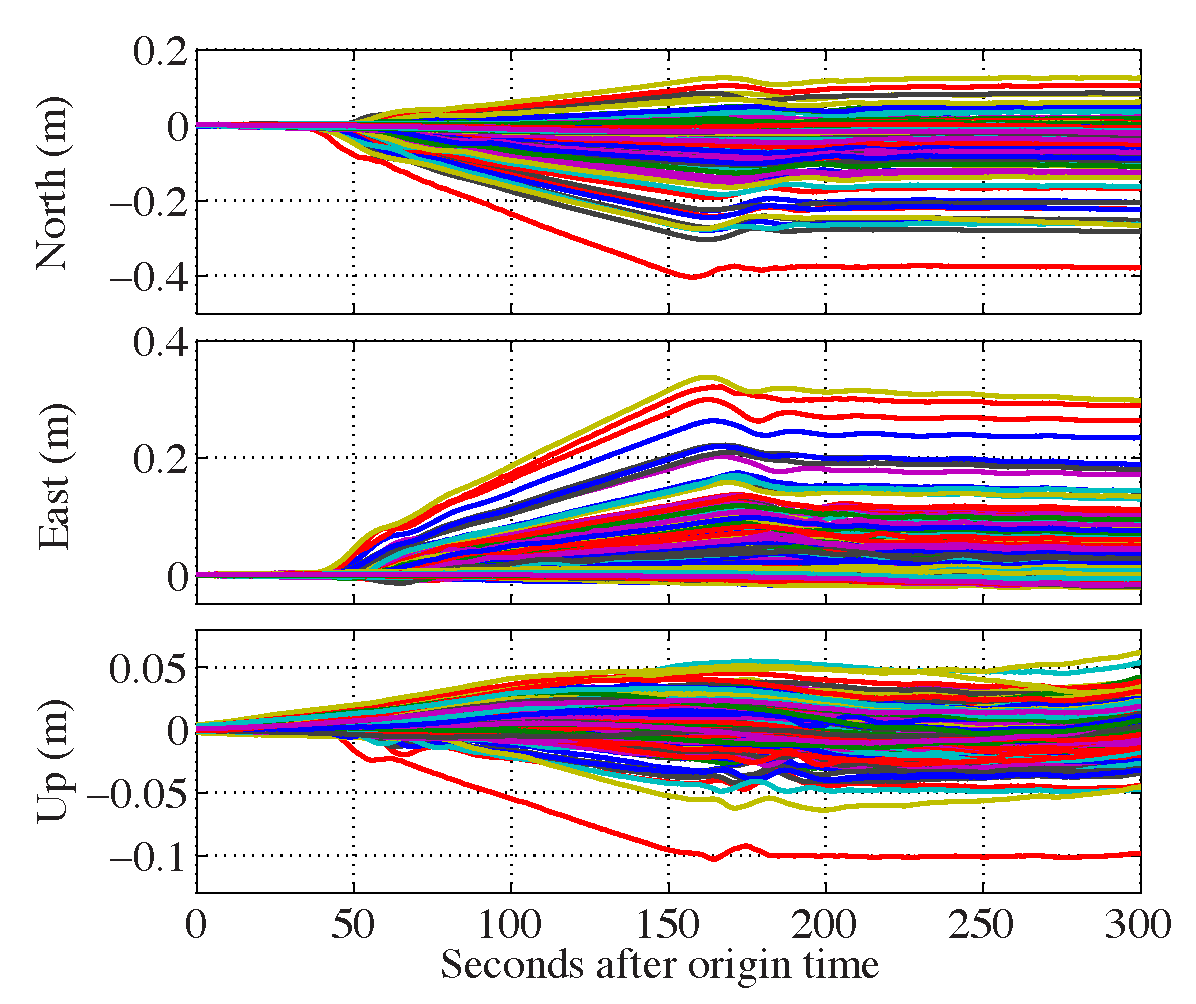
\includegraphics[width=0.88\linewidth]{./figures/ch3/toki_tseries.pdf}
    \caption[Tokachi-oki GPS time series]{First 300 s of displacement records at 355 GEONET stations with a 120 s moving average filter applied for the Tokachi-oki earthquake.}
  \label{fig_toki_tseries}
\end{figure}

Green's functions were computed from EDGRN on a 1 km horizontal and vertical grid using the four-layer velocity model employed by \citet{Yagi2004} for near source slip inversion (Table \ref{tb_toki_model}). This is a much denser coverage than the actual station distribution, thus, at any given station the resulting GF is the spline interpolation of the closest grid points. For this scenario we used a 3-D 3$^\circ\times$3$^\circ$ prism of gridpoints spaced at 0.2$^\circ$ and every 3km in depth between 3 and 60km centered around the mean latitude and longitude of the first stations to meet a detection criterion.

\begin{table}
\caption{Velocity model for the Tokachi-oki inversion}
\label{tb_toki_model}
\begin{tabular}{l r r r r}
\hline
Layer & $v_p$ & $v_s$ &Density&Thickness\\
 & (km/s) &( km/s) & (kg/m$^{3}$) & (km)\\
\hline
1 & 3.80 & 2.19 & 2.30 & 4.0\\
2 & 5.50 & 3.18 & 2.60 & 4.0\\
3 & 5.80 & 3.34 & 2.70 & 10.0\\
4 & 6.50 & 3.74 & 2.90 & 10.0\\
Half-space & 7.80 & 4.50 & 3.20 & $\infty$\\
\hline
\end{tabular}
\end{table}

We defined the criterion that displacements from 5 stations over the 15mm threshold are required to start the inversion; for the 2003 Tokachi-oki event this occurred at 43s after origin time. The results of the inversion are shown in Figures \ref{fig_toki_centroid_loc} and \ref{fig_toki_snaps}. Figure \ref{fig_toki_centroid_loc} shows the centroid determination as a function of time, Figure \ref{fig_toki_snaps} shows snapshots of the resulting CMT as well as the observed and synthetic horizontal displacements. Figure \ref{fig_toki_centroid_loc} shows that by 50 s a rough centroid location is available with oscillations between adjacent nodes. The magnitude reaches Mw 8.0 at 75s, with a 75\% variance reduction. However, as evidenced by the time series (Figure \ref{fig_toki_tseries}) the full coseismic offset has not yet occurred. The magnitude continues to grow and settles at 8.3 by 170s. The plot of the variance reduction also shows that at 200s (when the final offset is in place) the fit to the data is maximum (85\%) degrading towards the end of the inversion. Figure \ref{fig_toki_centroid_loc} shows the oscillation between adjacent nodes for the centroid solution and also indicate how by 65s a thrusting mechanism is already resolved although the magnitude is still underestimated. However, by 180s and onwards the inverted mechanism is close to that of the GCMT solution (http://www.globalcmt.org/).

\begin{figure}[!ht] 
  \centering
  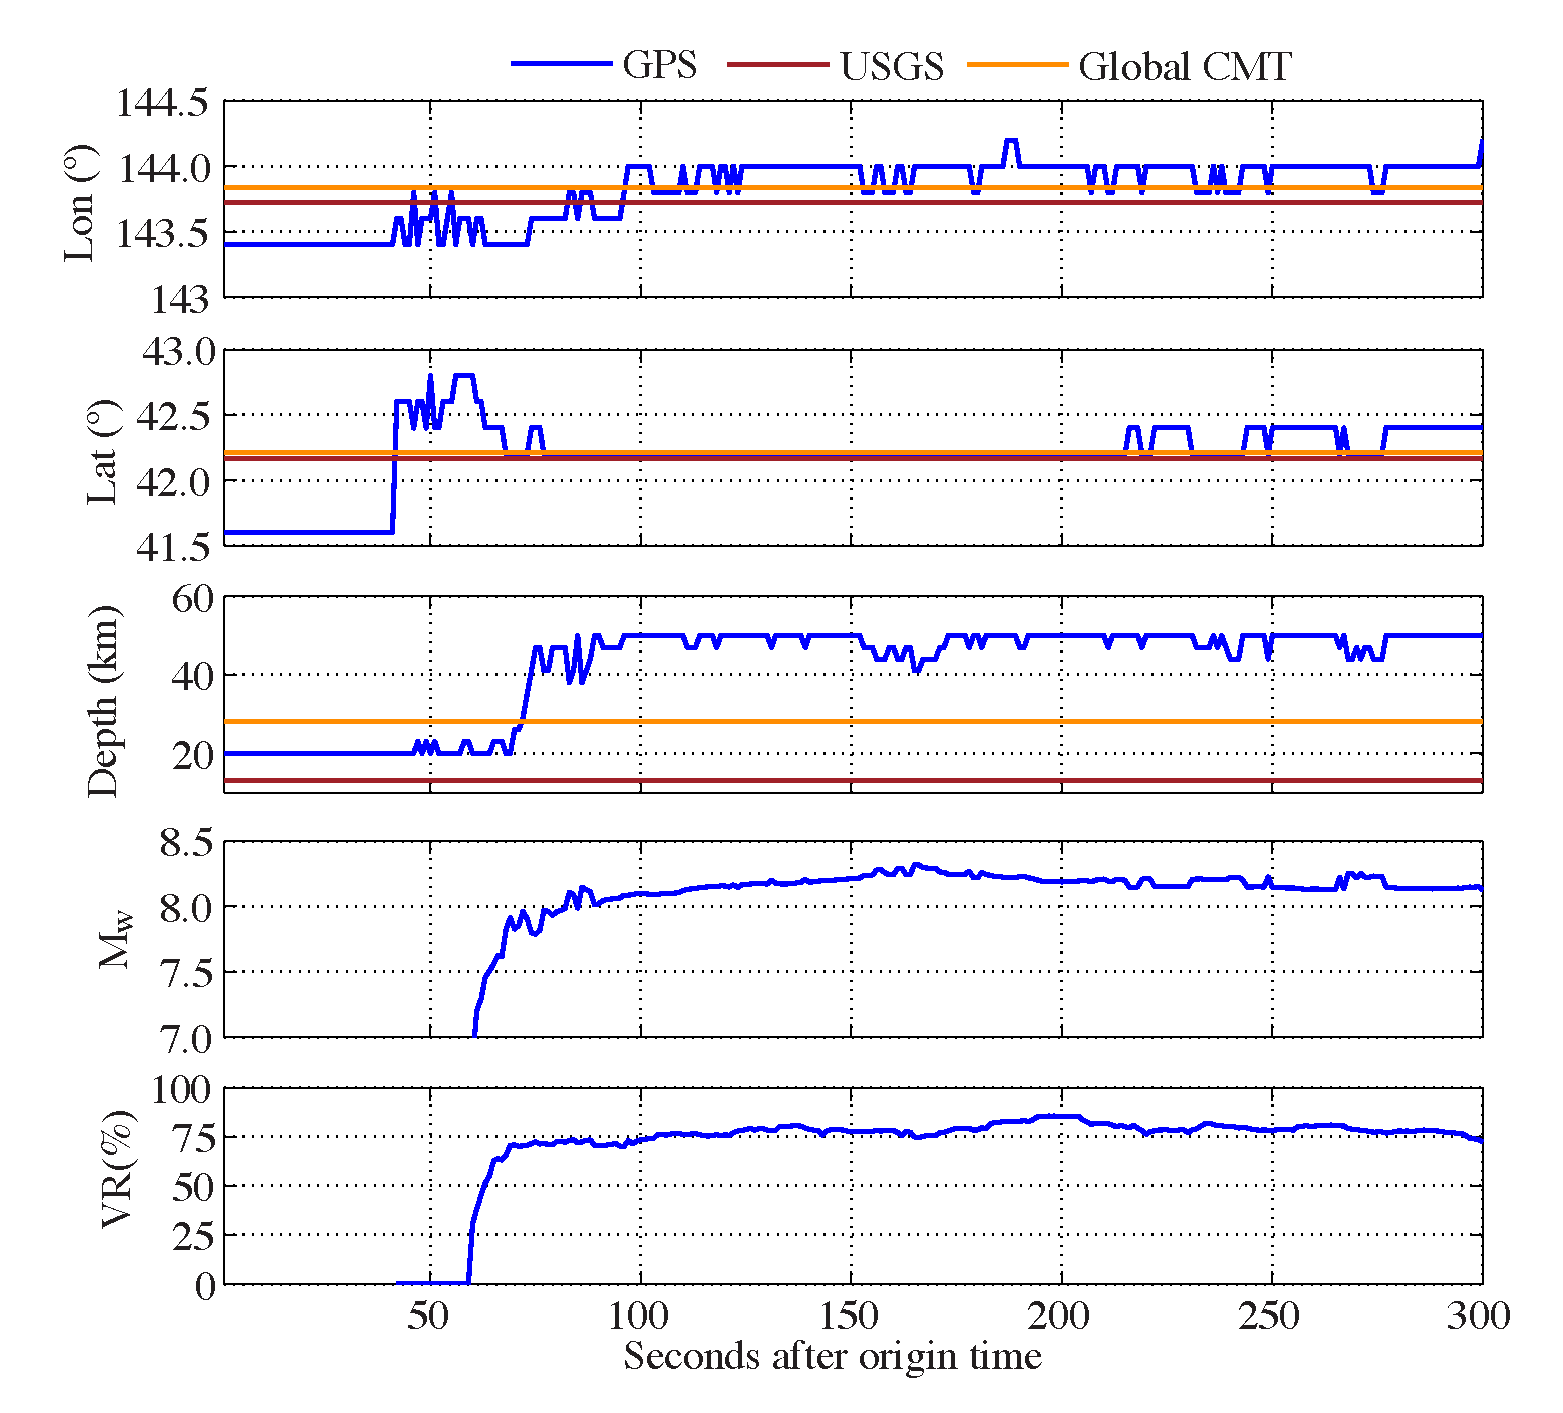
\includegraphics[width=0.88\linewidth]{./figures/ch3/toki_centroid_loc.pdf}
    \caption[Tokachi-oki inversion summary]{Summary of the inversion results for the Tokachi-oki earthquake. The top three panels are the centroid determination as a function of time compared to the location reported by the USGS and the Global Centroid Moment Tensor Project. The fourth panel is the computed magnitude and the fifth panel is the misfit (variance reduction).}
  \label{fig_toki_centroid_loc}
\end{figure}

\begin{figure}[!ht] 
  \centering
  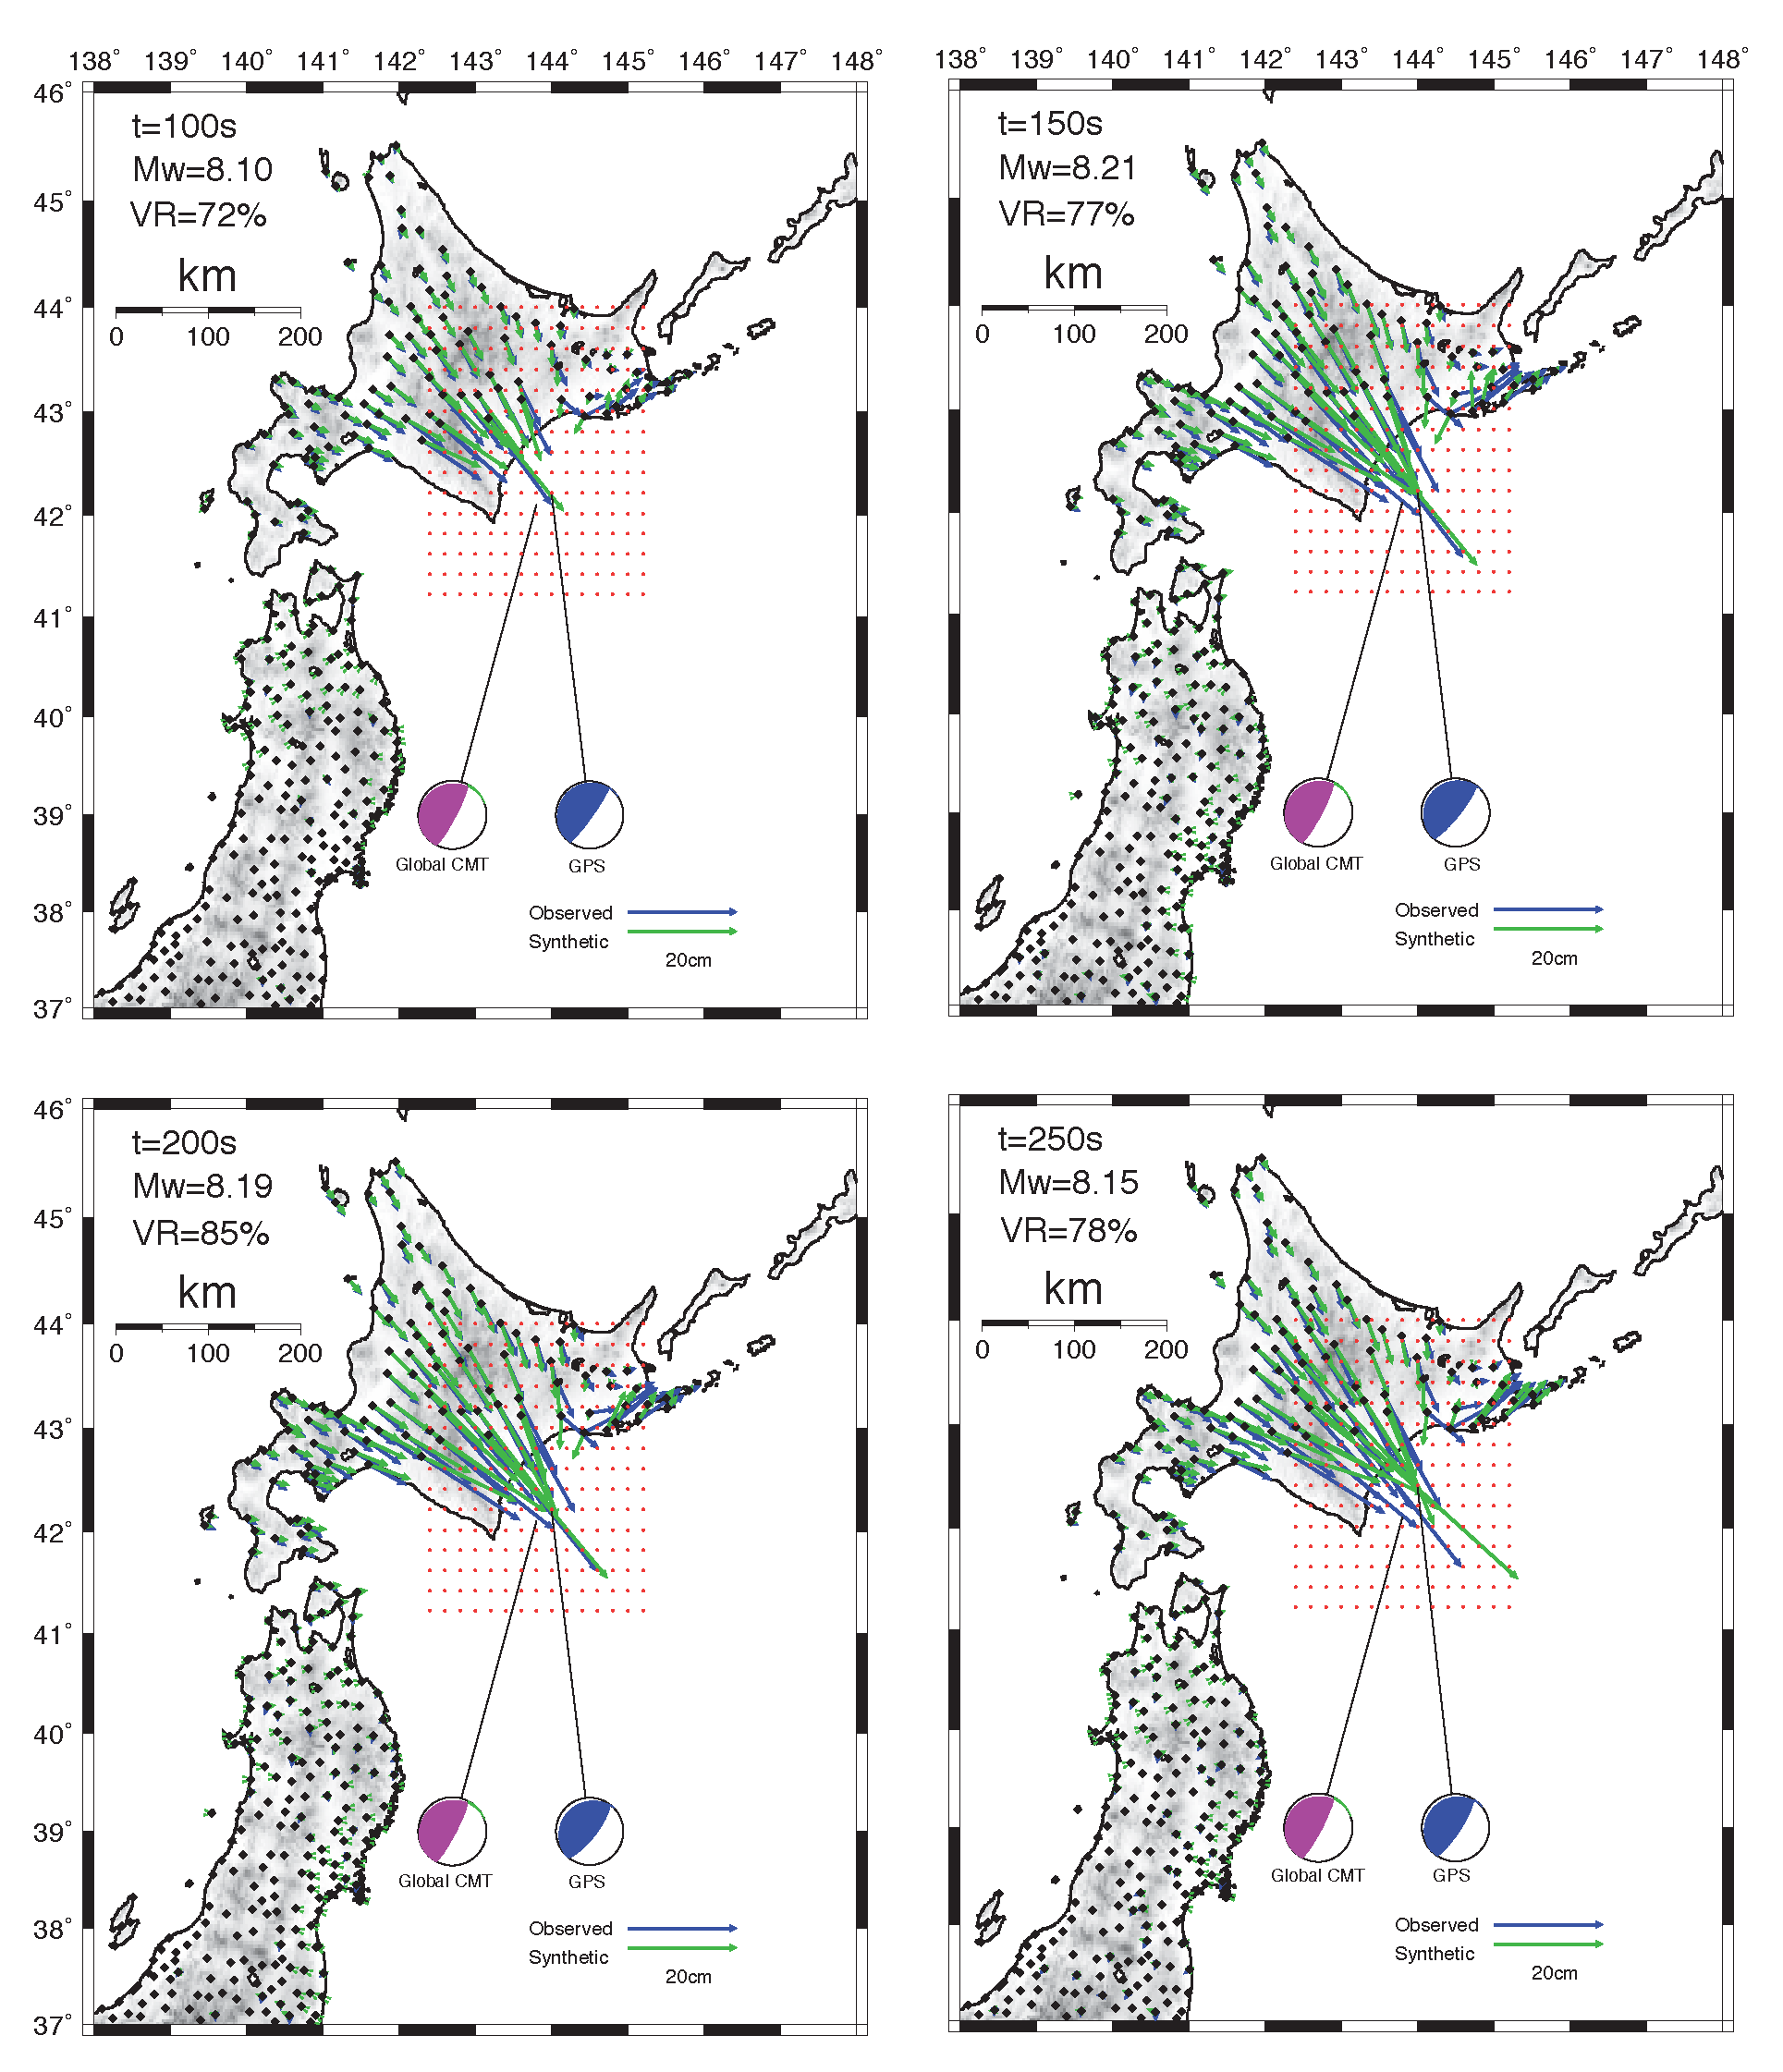
\includegraphics[width=0.99\linewidth]{./figures/ch3/toki_snaps.pdf}
    \caption[Tokachi-oki inversion snapshots]{Snapshots of the inversion results comparing the Global CMT result with the replayed GPS real time inversion for the 2003 Mw 8.3 Tokachi-oki earthquake. Mw is the moment magnitude and VR the variance reduction. The red dots indicate the inversion nodes of the 3$^\circ$ by 3$^\circ$ grid used for the grid search. Also shown is the comparison between the observed (blue) and modeled (green) horizontal offsets. }
  \label{fig_toki_snaps}
\end{figure}

To further evaluate the quality of the solution we extracted the strike, dip and rake of the nodal planes from the moment tensor solution every second by decomposing it into its best double couple. The results are shown in Figure \ref{fig_toki_stdiprake}  and compared to the GCMT results. They illustrate that the geometrical parameters of the best double couple are well determined at 65s, before the full coseismic deformation occurs, and remain fairly similar to the post-processed GCMT solution throughout. Furthermore the size of the CLVD is fairly small throughout the inversion, never exceeding $\epsilon=0.05$.

\begin{figure}[!ht] 
  \centering
  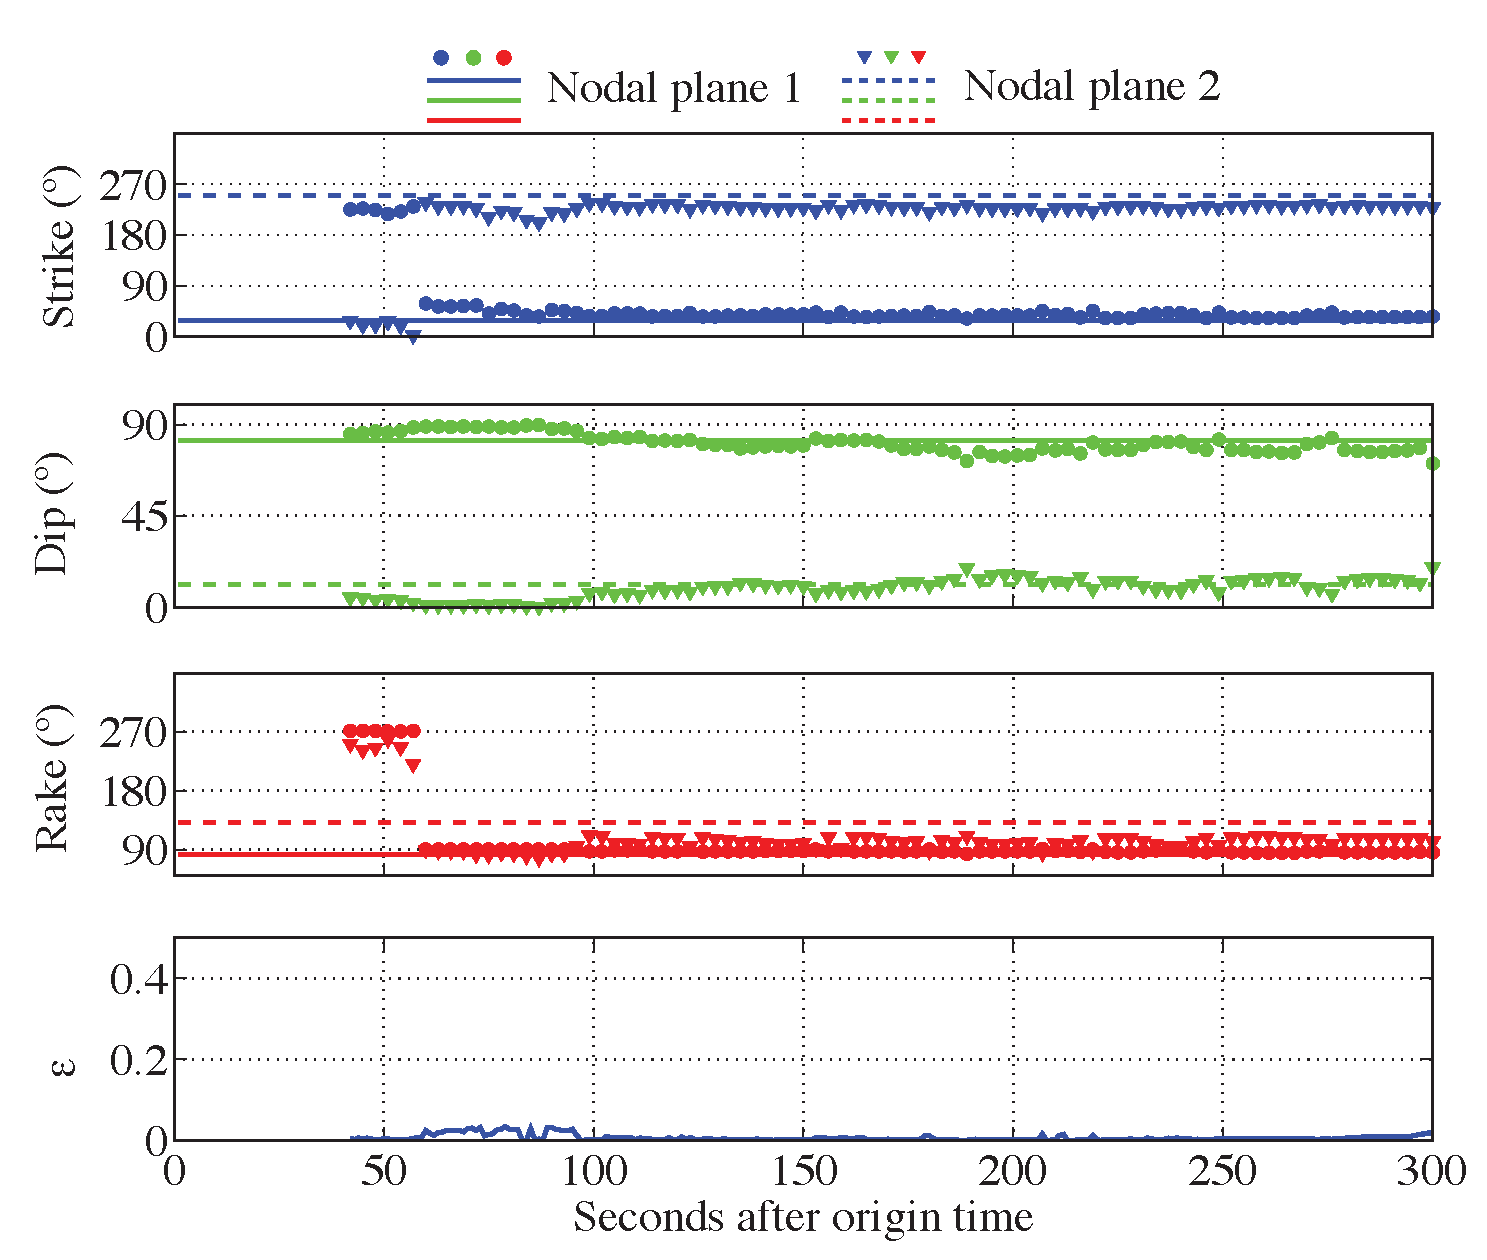
\includegraphics[width=0.99\linewidth]{./figures/ch3/toki_stdiprake.pdf}
    \caption[Tokachi-oki time evolution of best double-couples]{Geometrical parameters of the best double couple solution extracted from the moment tensor inversion and compared to the global CMT post-processed result. Data for both nodal planes (NP1 and NP2) are plotted at 3s intervals for clarity. $\epsilon$ is defined in Equation \ref{eq_epsilon}. Data starts at 43s when enough stations detect an offset.}
  \label{fig_toki_stdiprake}
\end{figure}

\subsubsection{The 2010 Mw 7.2 El Mayor Cucapah Earthquake}

The 2010 Mw 7.2 El Mayor-Cucapah earthquake ruptured roughly 120km of the Pacific-North America plate boundary in northern Baja California, Mexico. The rupture was complex possibly starting with a normal faulting event followed by simultaneous normal and right lateral faulting \citep{hauksson2011}. The rupture plane showed evidence of a warped fault, was bilateral and the rake changed along strike away from the epicenter from pure strike slip to a mixture of strike slip and dip slip motion \citep{wei2011}. 

Displacements at a 1Hz sampling rate were estimated in a simulated real-time mode for 105 stations of the California Real Time Network in southern California as described in Chapter 2. As in the first event, we applied the 120 s moving average filter, at each epoch we exclude stations with horizontal offsets smaller than 15 mm (Figure \ref{fig_elmay_tseries}), and started the inversion process when 5 stations detected motion over the threshold; at 41s after origin time for the 2010 El Mayor-Cucapah event. The horizontal coseismic offsets are apparent at the stations closer to the source by 150s in both components although some shaking is still visible in the form of small oscillations. By 200s the shaking ceases and only the offset remains. Offsets are not easily discernible in the vertical components, which remain noisy throughout. This is reasonable since this earthquake produced only small vertical offsets of $\sim$5mm from the stations closer to the source as estimated, for example, from the more accurate, standard 24 hour displacement time series.

\begin{figure}[!ht] 
  \centering
  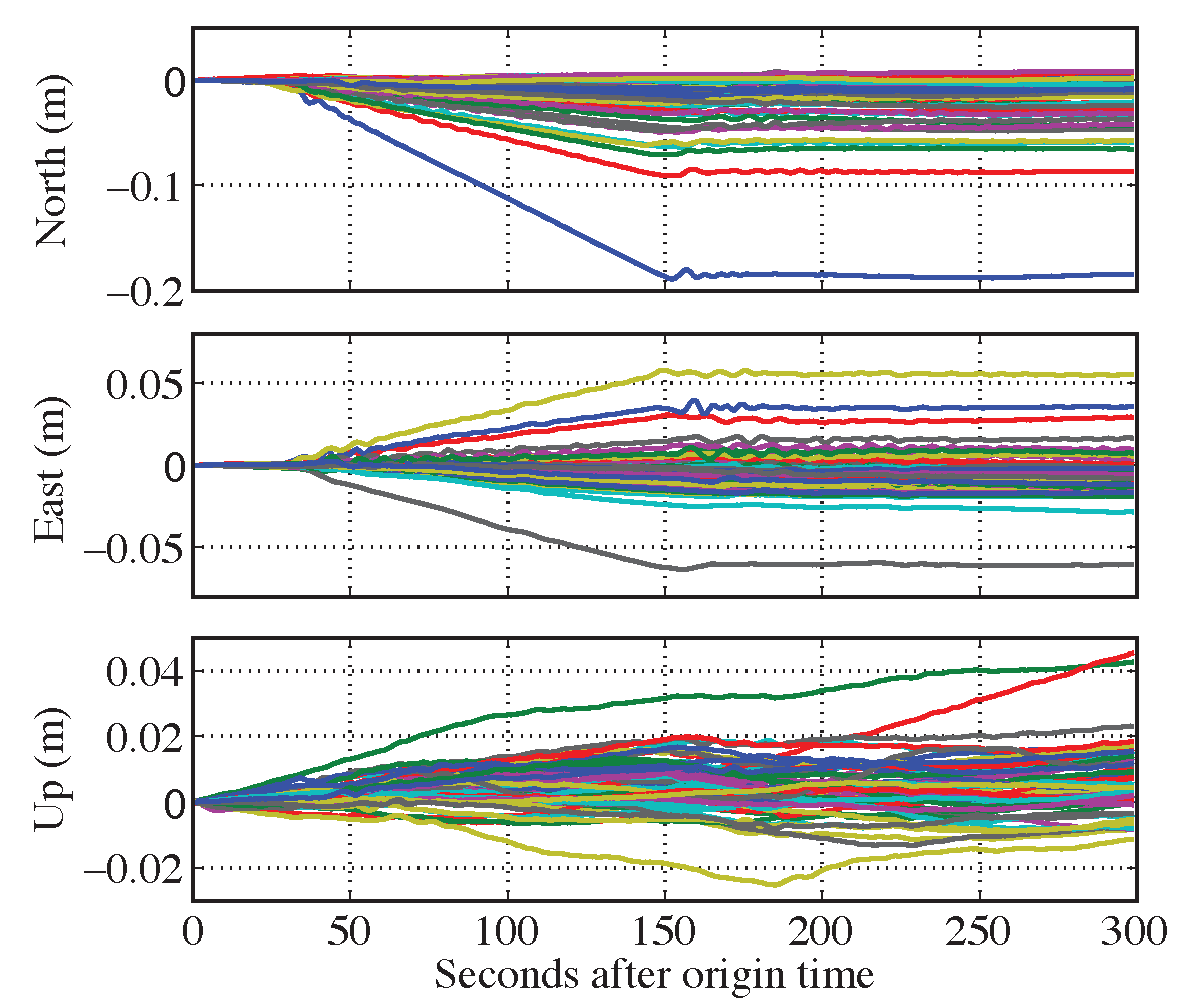
\includegraphics[width=0.88\linewidth]{./figures/ch3/elmay_tseries.pdf}
    \caption[El Mayor-Cucapah GPS time series]{300s of displacement records at 50 of the 105 CRTN stations that exceeded the 15mm threshold with a 120s moving average filter applied for the 2010 Mw 7.2 El Mayor-Cucapah earthquake}
  \label{fig_elmay_tseries}
\end{figure}

The seismic velocity model used in the inversion is obtained from a simplification of the California Community Velocity Model version 4 (CVM4) \citep{kohler2003}. The structure in this zone is highly heterogeneous so our model is an average of the grid with corners (117$^\circ$W, 32$^\circ$N) and (115$^\circ$W, 34$^\circ$N). We assume a constant Moho depth, which is taken as the mean value inside the grid.  We define 4 layers between the Moho and the free surface, and assume a half space below the Moho (Table \ref{tb_elmay_model}). The GFs for this model are computed at 1 km horizontal and vertical intervals with EDGRN and as before, at a particular station the GF is the result of the spline interpolation of the closest grid points.

\begin{table}
\caption{Velocity model for the El Mayor-Cucapah inversion}
\label{tb_elmay_model}
\begin{tabular}{l r r r r}
\hline
Layer & $v_p$ & $v_s$ &Density&Thickness\\
 & (km/s) &( km/s) & (kg/m$^{3}$) & (km)\\
\hline
1 & 4.14 & 2.18 & 2.33 & 4.16\\
2 & 5.73 & 3.34 & 2.67 & 4.16\\
3 & 6.37 & 3.66 & 2.80 & 8.32\\
4 & 6.64 & 3.74 & 2.87 & 8.32\\
Half-space & 7.69 & 4.38 & 3.218 & $\infty$\\
\hline
\end{tabular}
\end{table}

In order to avoid the use of a library of fault surfaces we place a rectangular 3$^\circ$ by 3$^\circ$ grid of inversion nodes around the mean latitude and longitude of the first 5 stations to detect 15mm of horizontal motion and spaced at 0.1$^\circ$ in latitude and longitude and 2km in depth from 2-20km. As before, we prefer an L1-norm inversion. Figure \ref{fig_elmay_centroid_loc} shows a summary of the centroid determination and magnitude results of the inversion. The centroid is well located by 50s. After 50s the centroid location oscillates between adjacent nodes; the depth oscillates between 2 and 8km before settling at 2km by 280s. The variance reduction is maximum ($\sim$85\%) by 150s and worsens slightly towards the end of the inversion, the style of faulting is not well resolved until ~150s (Figures \ref{fig_elmay_snaps} and \ref{fig_elmay_stdiprake}). The moment magnitude estimate reaches 7.2 by 60s but continues to grow and oscillates between 7.0 and 7.5, before becoming fairly stable at 7.2 by 160s.

\begin{figure}[!ht] 
  \centering
  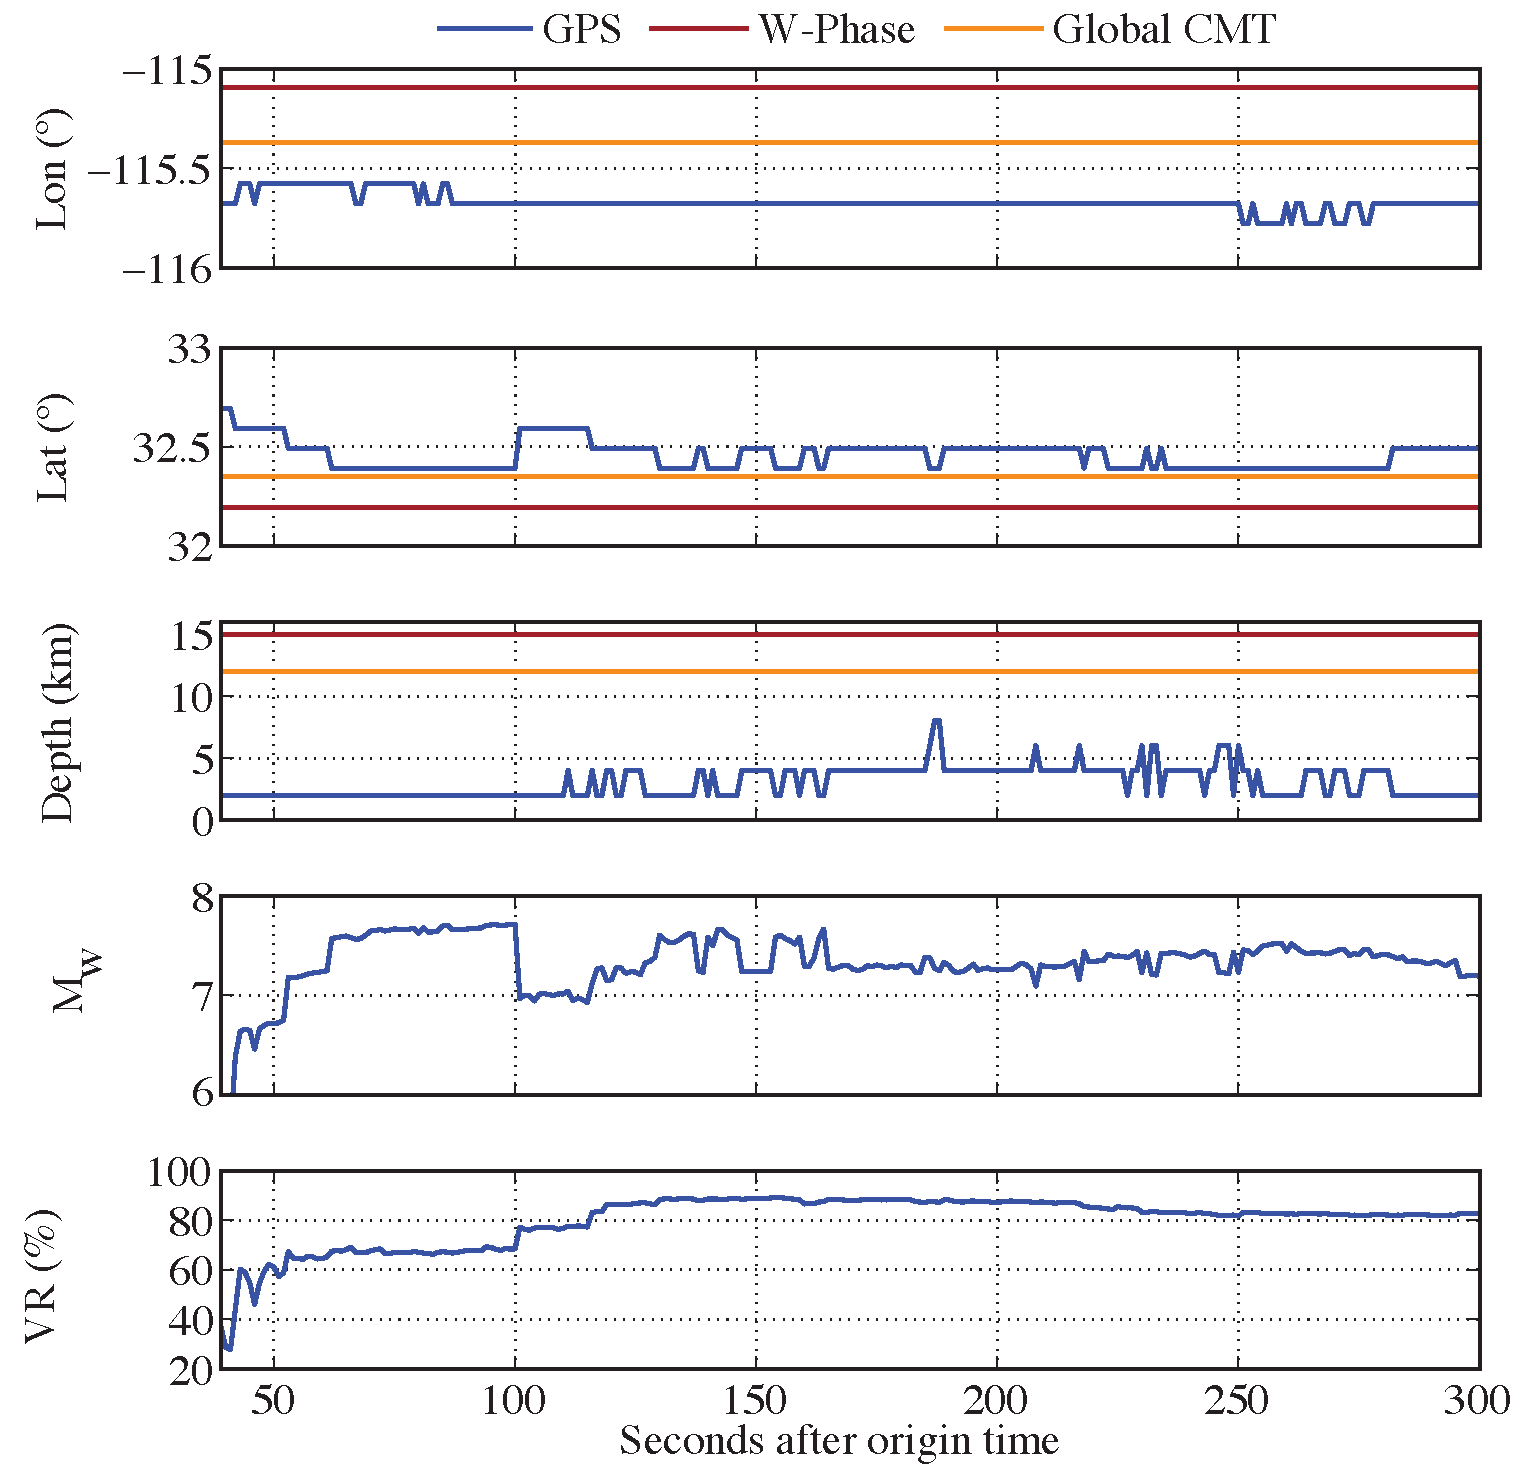
\includegraphics[width=0.88\linewidth]{./figures/ch3/elmay_centroid_loc.pdf}
    \caption[El Mayor-Cucapah inversion summary]{Summary of the inversion results for the El Mayor-Cucapah earthquake. The top three panels are the centroid determination as a function of time compared to the location reported by the USGS W-Phase inversion and the Global Centroid Moment Tensor Project. The fourth panel is the computed magnitude and the fifth panel is the misfit (variance reduction).}
  \label{fig_elmay_centroid_loc}
\end{figure}

\begin{figure}[!ht] 
  \centering
  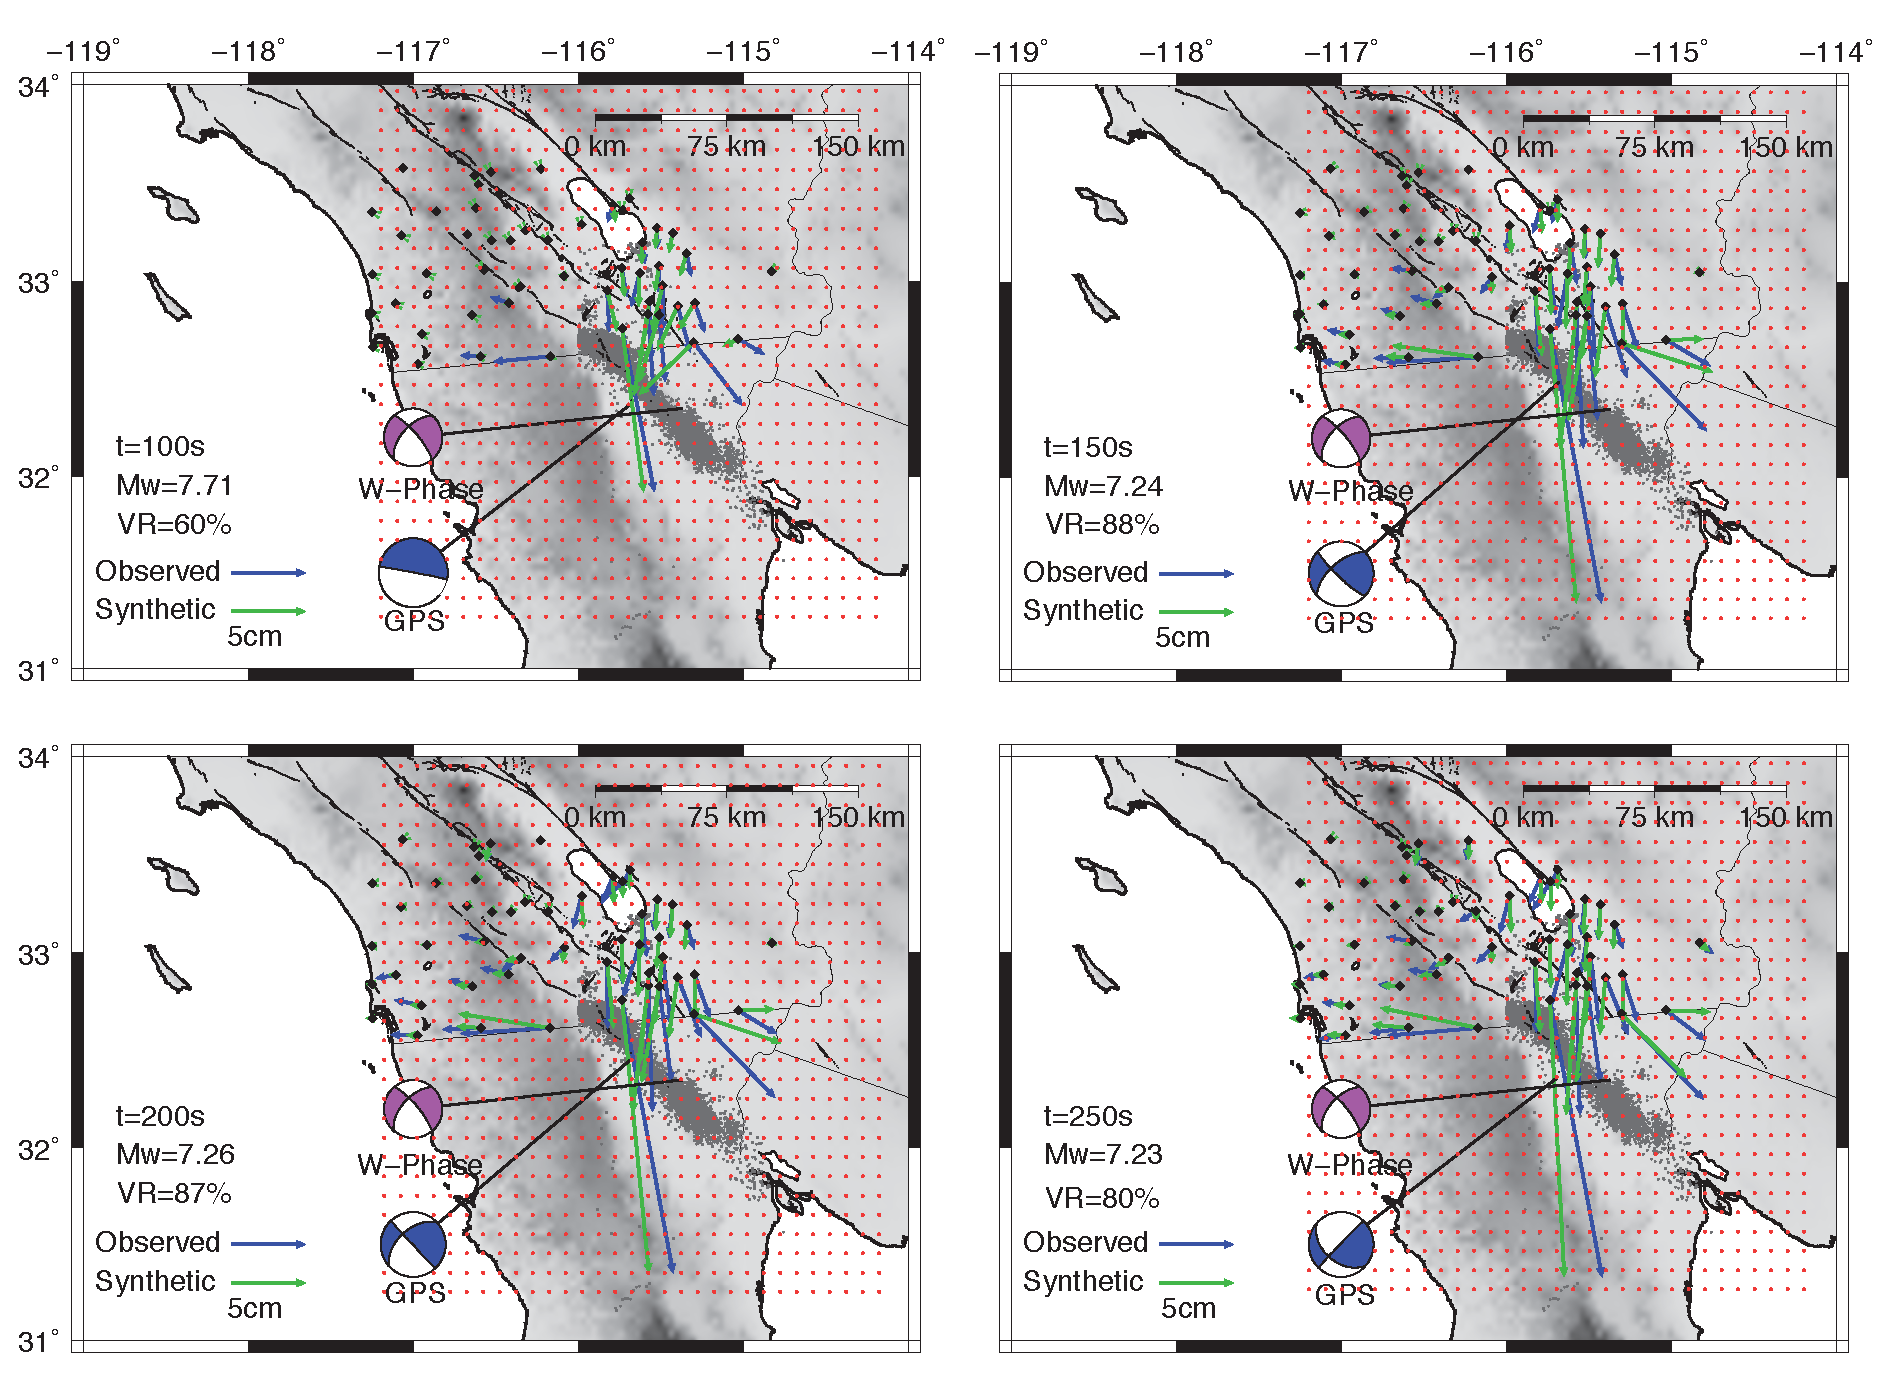
\includegraphics[width=0.99\linewidth]{./figures/ch3/elmay_snaps.pdf}
    \caption[El Mayor-Cucapah inversion snapshots]{Snapshots of the inversion results for the El Mayor Cucapah earthquake comparing the USGS W phase result with the GPS real-time inversion. Also shown is the comparison between the observed and modeled horizontal offsets. The red dots indicate the nodes used for the grid search, dark grey dots are one year of aftershocks reported by the Southern California Seismic Network (www.data.scec.org) and black lines indicate Quaternary faults in southern California.}
  \label{fig_elmay_snaps}
\end{figure}

The focal mechanisms display some interesting characteristics during the inversion; Figure \ref{fig_elmay_snaps} shows snapshots of the inversion and centroid location at 50s intervals and Figure \ref{fig_elmay_stdiprake} shows the strike, dip and rake of the best double couple solutions. By 120s the best double couple solution is almost pure strike-slip with strike and dip very similar to the W phase solution and a centroid $\sim$30km from the W phase centroid. The strike of both nodal planes remains fairly consistent throughout as does the rake and the dip of the first nodal plane. However the dip of the second nodal plane oscillates throughout the inversion. Furthermore, the size of the CLVD component is quite large with a mean value of 0.25 during the inversion period. This is consistent with the observations of \citet{hauksson2011} who obtain similar results from post-event W phase inversions and analysis of satellite geodesy data \citet{wei2011} which indicate that a large CLVD reflects source complexity and is a real signal.

\begin{figure}[!ht] 
  \centering
  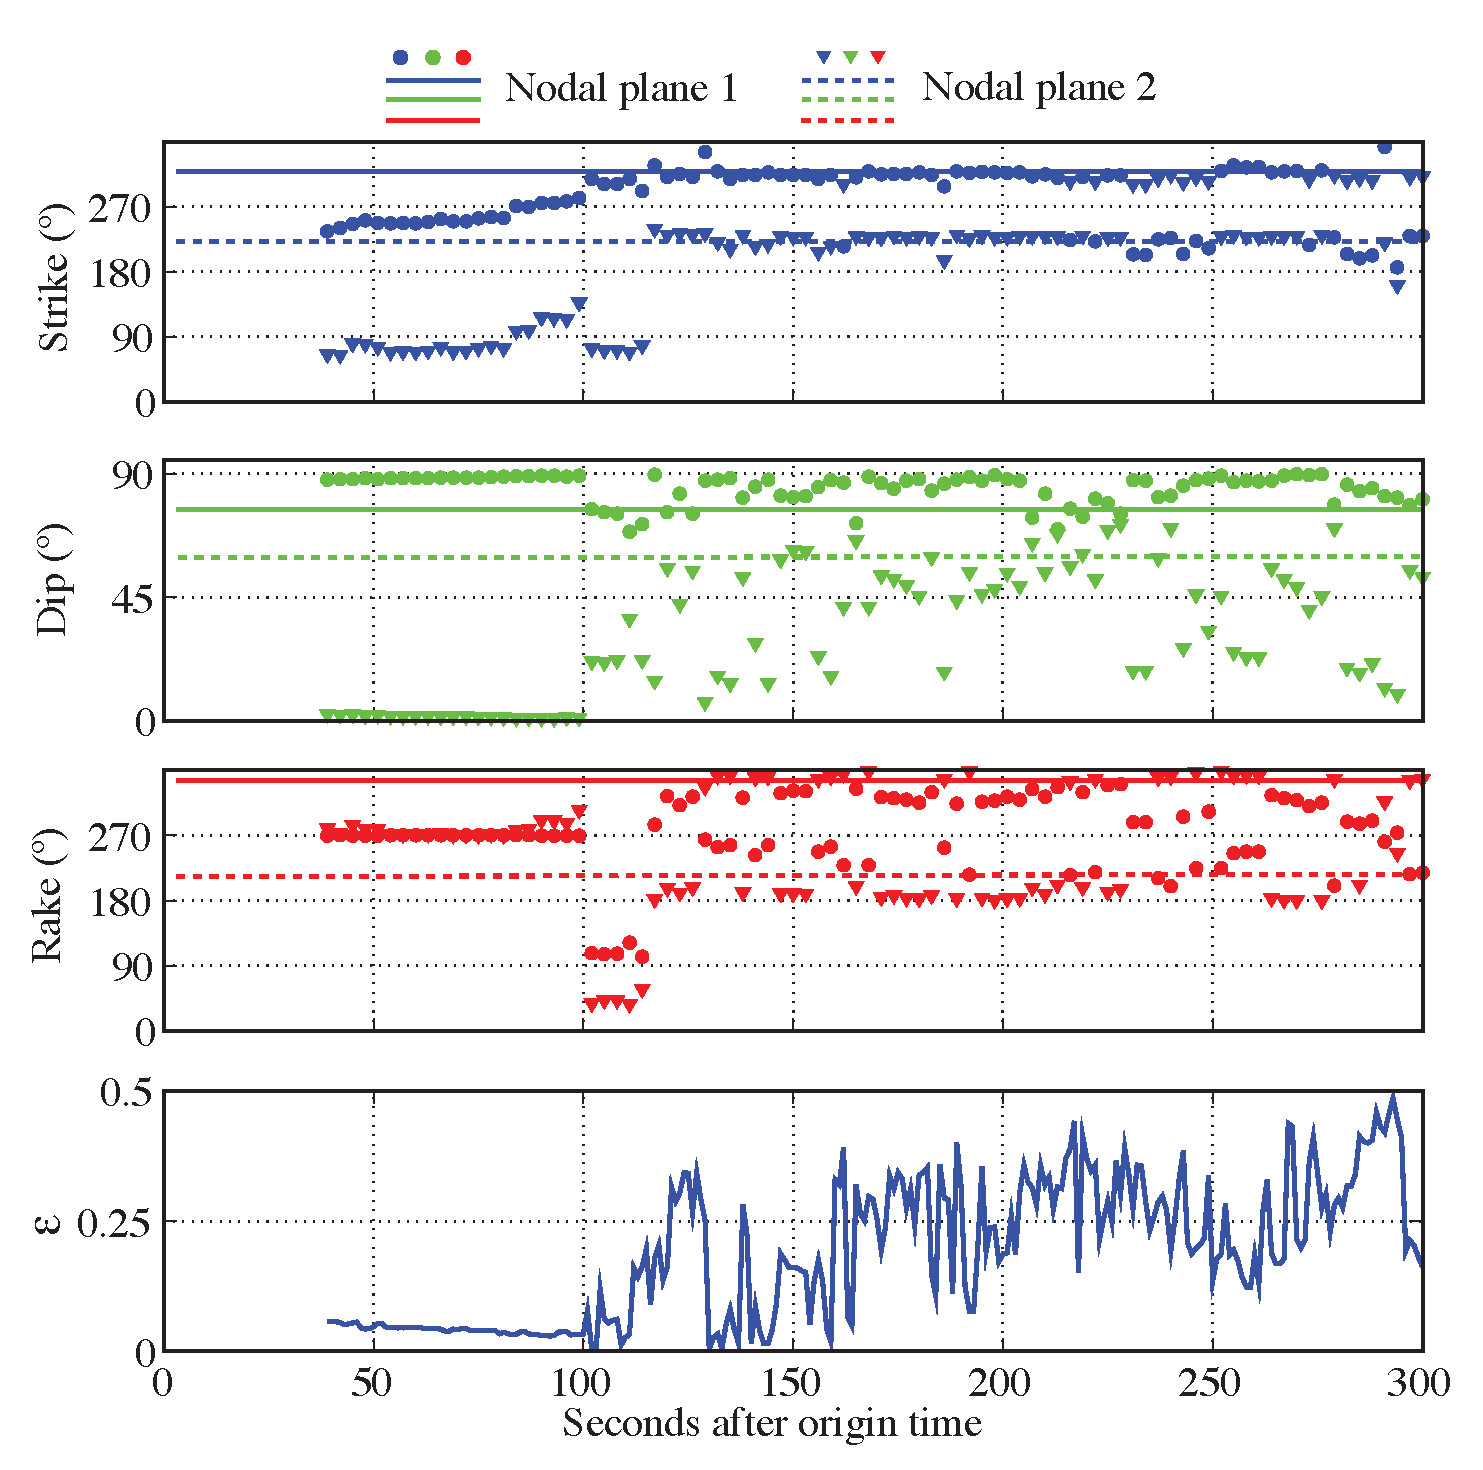
\includegraphics[width=0.99\linewidth]{./figures/ch3/elmay_stdiprake.pdf}
    \caption[El Mayor-Cucapah time evolution of best double-couples]{Geometrical parameters of the best double couple solution extracted from the moment tensor inversion and compared to the USGS W phase post-processed result for the 2010 El Mayor-Cucapah earthquake. Data for both nodal planes (NP1 and NP2) are plotted at 3s intervals for clarity. $\epsilon$ is defined in Equation \ref{eq_epsilon}. Data starts at 41s when enough stations detect an offset.}
  \label{fig_elmay_stdiprake}
\end{figure}

\subsection{Final Point Source Solutions}

We have shown that the final CMT solution is quickly obtained after the end of the rupture process as soon as the full permanent deformation has been discerned.  The convergence to the final CMT solution is illustrated in Figure \ref{fig_final_inversion} for both earthquakes. The procedure in initiated as described earlier when 5 stations have a total horizontal displacement that exceeds the 15mm threshold.  We refer to this instant as the time of first detection $t_d$; it is the time at which we launch the procedure to determine the final coseismic offsets. The mean latitude and longitude of the 5 GPS stations is computed, and a 3$^\circ$ by 3$^\circ$ grid around that value is defined. The pre-computed GFs are spline interpolated to compute values at each grid point. A grid search is initiated to determine the event centroid. In addition to the 120s moving average computed for the total horizontal displacements.  We also compute the variance of 20 samples previous to the current epoch (Figure \ref{fig_final_inversion}a and \ref{fig_final_inversion}e); as the offset grows, the variance will be high and when the displacement stabilizes to its final level the variance will diminish and stabilize. Only the station with the maximum horizontal displacement is considered at this point of the analysis. At each epoch, the station that obeys this constraint is tracked; it can change from epoch to epoch depending on the location of the network with respect to the earthquake source. Thus, the displacement traces shown in Figure \ref{fig_final_inversion} (a, e) could be a composite of several stations. The variance at each epoch is computed over the previous 20 samples (or the previous 20s for 1Hz data). At every instant we track whether the observed variance is the maximum observed one  ($s^2_{max}$) up to that given point (the time of maximum variance is $t_{max}$). Simultaneously, we track whether the variance has dropped below an empirically set threshold $p\cdot s^2_{max}$ where $p=0.25$. The epoch where that threshold is breached is time $t_1$ and we assume this to be the instant when the final offset at the station with the maximum horizontal displacement has been reached. Evidently some error is incurred here from stations not yet developing the full offset, but after experimenting with values of $p$ ranging from 0.01 to 0.5, and comparing with post-processed inversions we conclude that 0.25 is optimum. A high value for $p$ detects the final offset earlier but does not allow for enough stations to have reached a final offset, conversely a low value of $0.1$ waits an unnecessarily long time for the final offset solution.

\begin{figure}[!ht] 
  \centering
  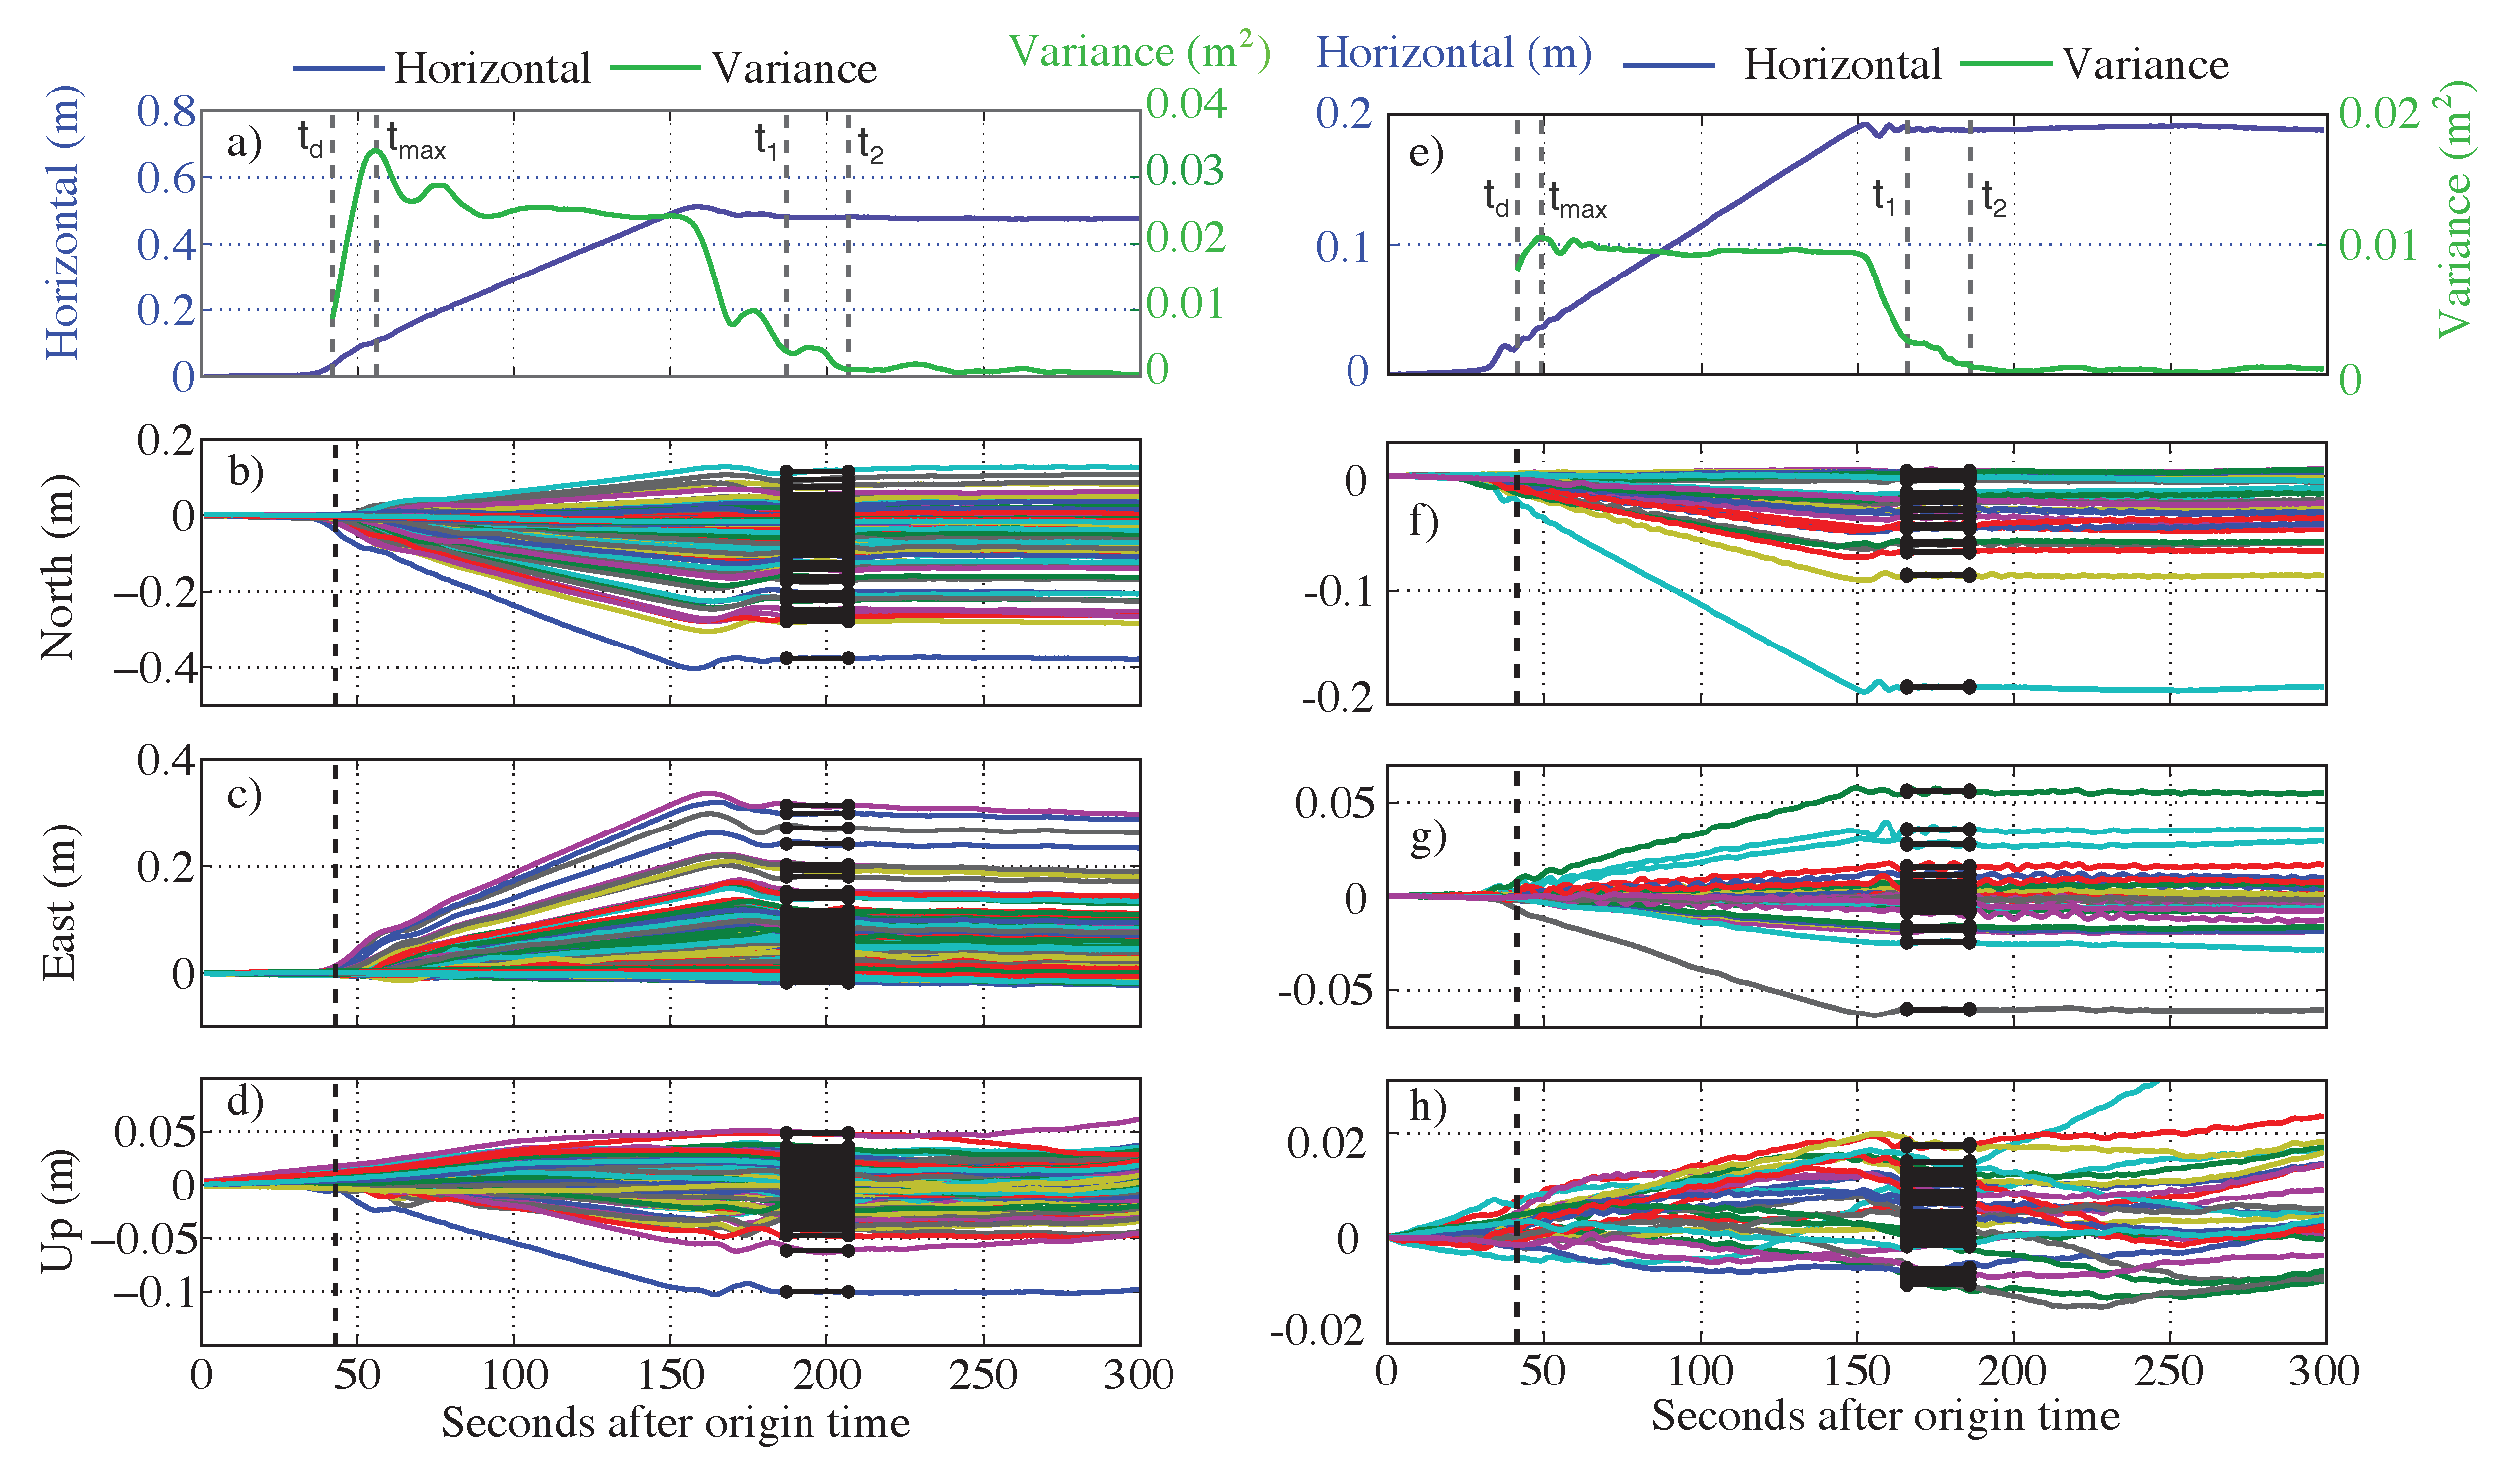
\includegraphics[width=0.99\linewidth]{./figures/ch3/final_inversion.pdf}
    \caption[Detection of final coseismic offsets]{a) Maximum horizontal displacement and variance function used for determination of final offsets for the Tokachi-oki earthquake (see text for detailed description). $t_d$ is the time at which anomalous motion is detected, $t_{max}$ is the time of maximum variance, $t_1$ is the time when the variance function drops to 25\% of the maximum value and defines the start of the averaging interval and $t_2$ is 20s after $t_1$ and is the end of the averaging interval and the time at which a final solution is available. b)-d) Final offsets determined for the 3 directions of motion for the Tokachi-oki event. d) Maximum horizontal displacement and variance function used for determination of final offsets for the El Mayor-Cucapah earthquake (see text for detailed description); $t_d$, $t_{max}$, $t_1$ and $t_2$ have the same definition as in 9a. f)-h) Final offsets determined for the 3 directions of motion for the El Mayor-Cucapah event}
  \label{fig_final_inversion}
\end{figure}

\begin{figure}[!htb] 
  \centering
  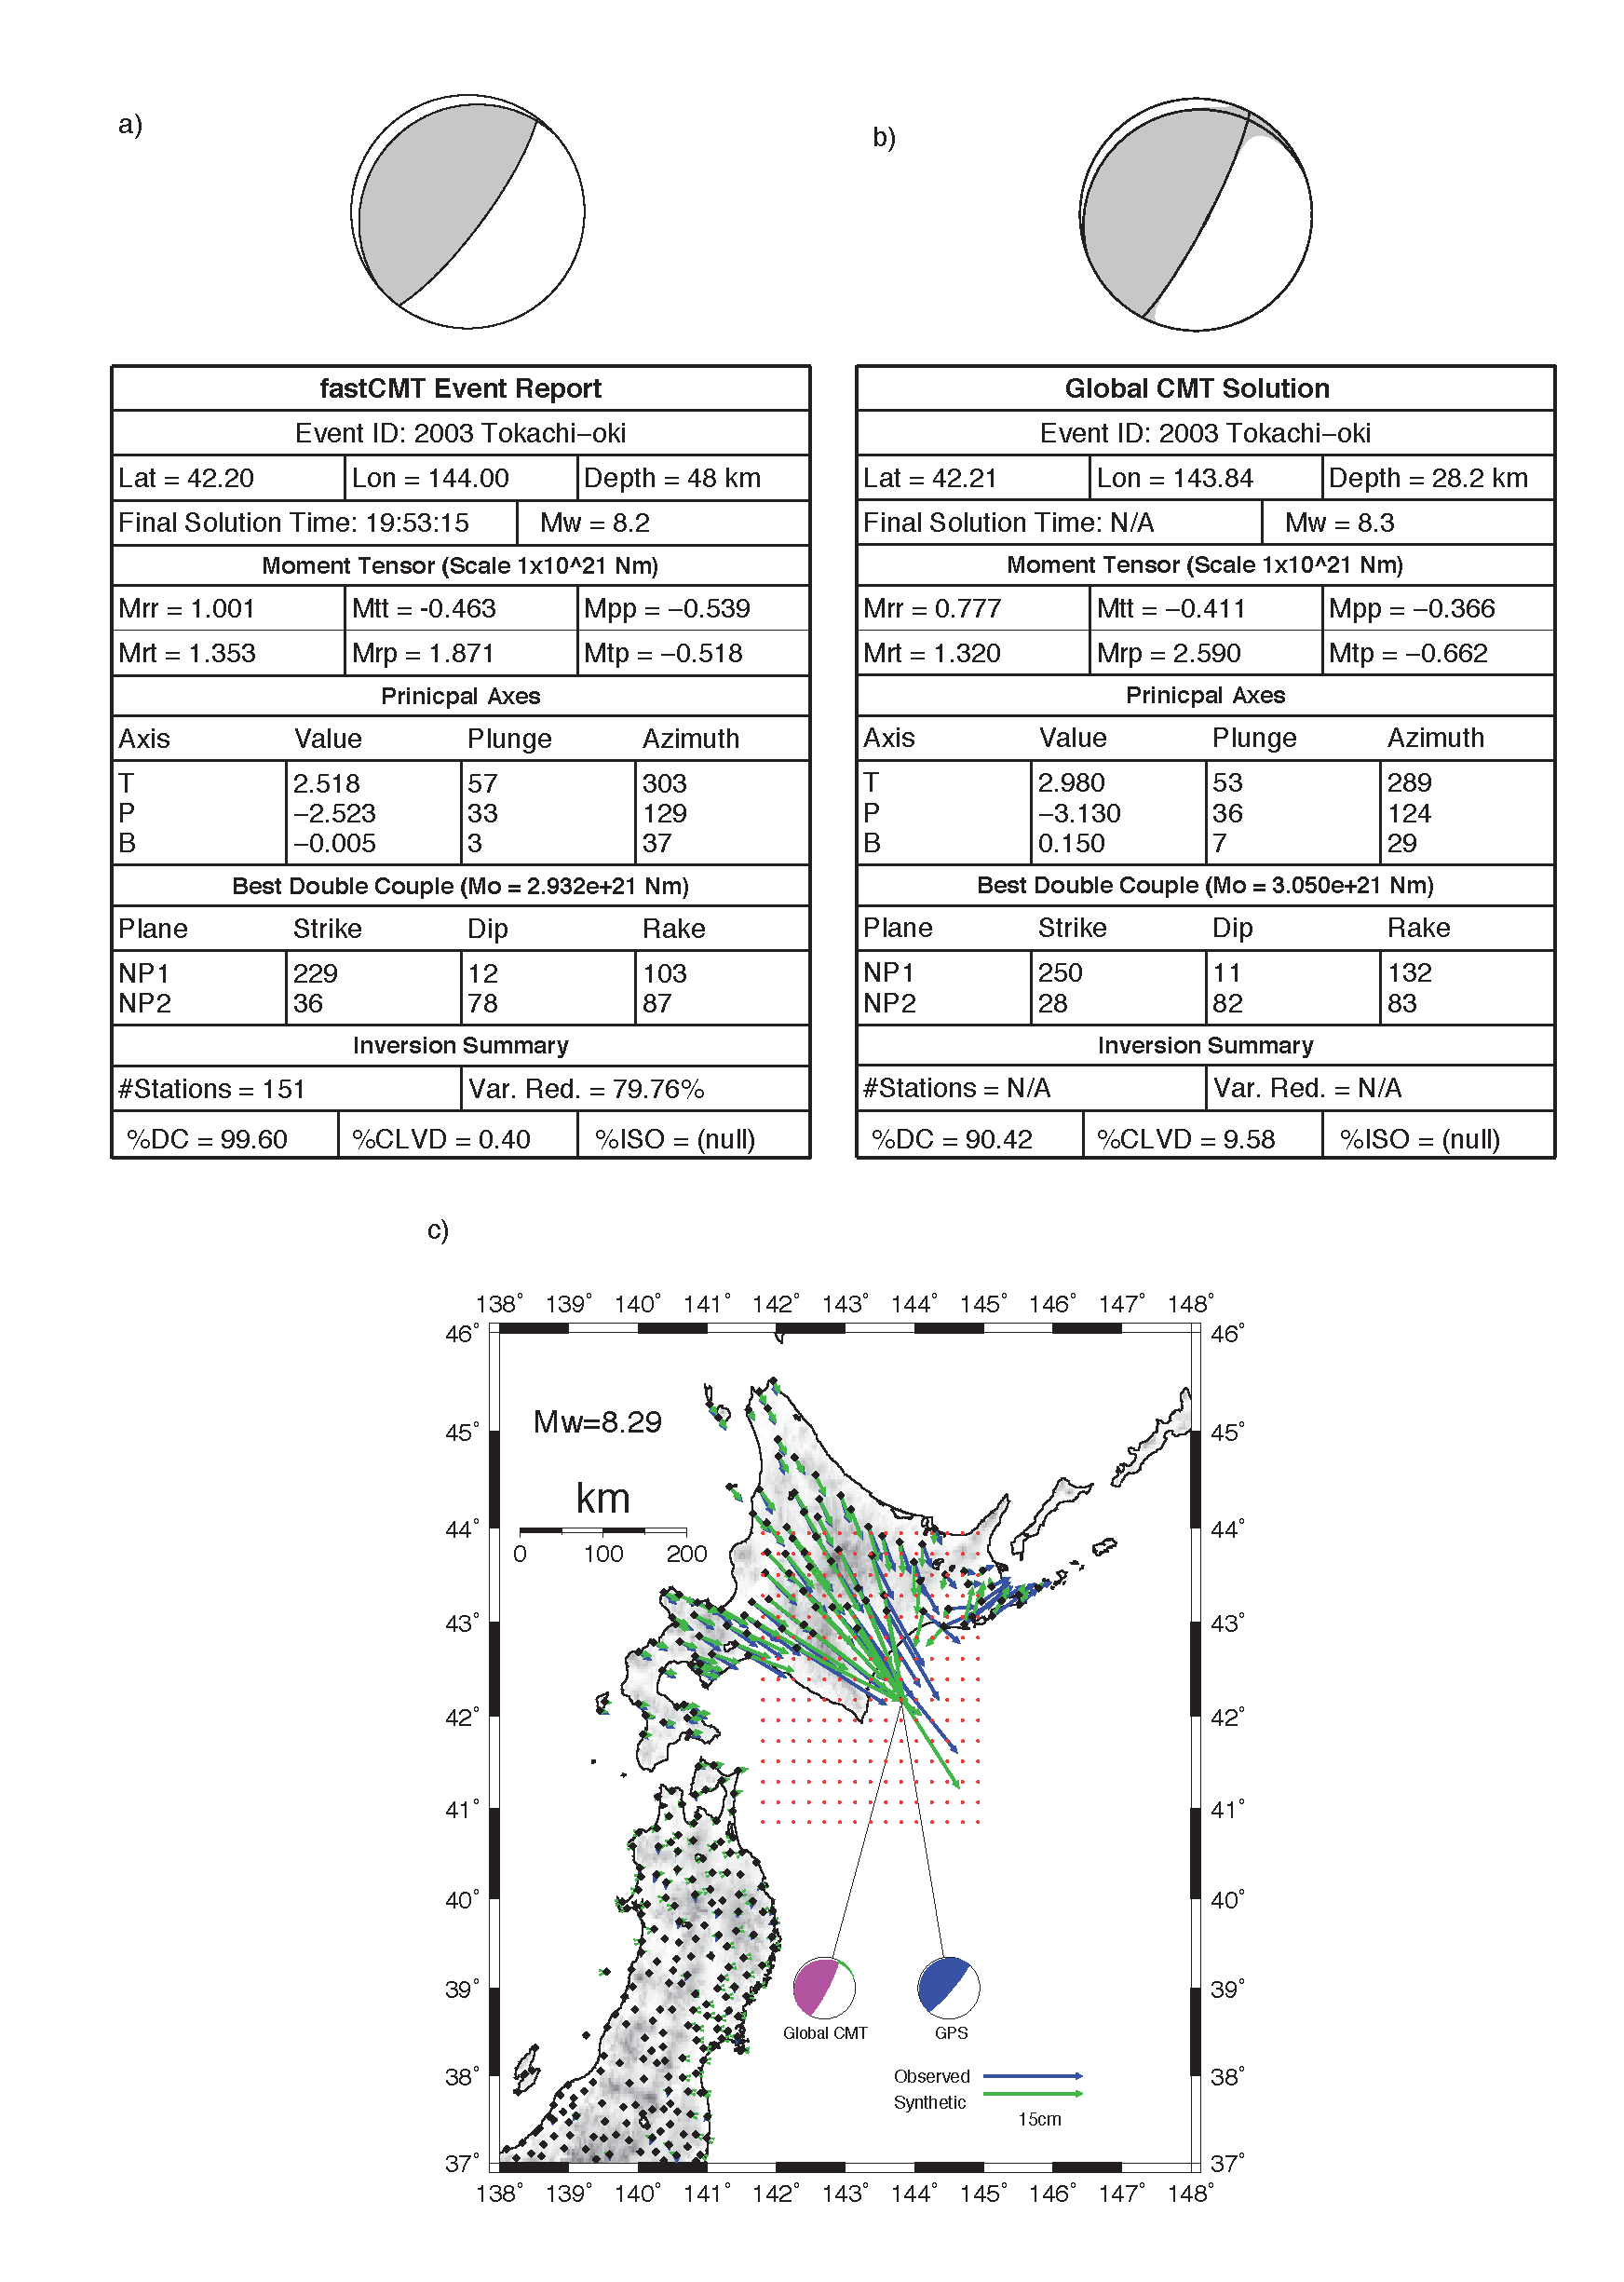
\includegraphics[width=0.9\linewidth]{./figures/ch3/toki_final.pdf}
    \caption[Tokachi-oki final inversion results]{Detailed comparison between the a) fastCMT and b) GCMT results for the Tokachi-oki event. c) Comparison between the best double-couple solutions as computed in (a) and (b) and the synthetic and observed displacements of (a)}
  \label{fig_toki_final}
\end{figure}

\begin{figure}[!htb] 
  \centering
  \includegraphics[width=0.9\linewidth]{./figures/ch3/elmay_final.pdf}
    \caption[El Mayor-Cucapah final inversion results]{Detailed comparison between the a) fastCMT and b) USGS W-Phase results for the El Mayor-Cucapah event. c) Comparison between the best double-couple solutions as computed in (a) and (b) and the synthetic and observed displacements of (a)}
  \label{fig_elmay_final}
\end{figure}

As evidenced by Figure \ref{fig_toki_stdiprake} and \ref{fig_elmay_stdiprake} there is still a considerable amount of scatter in the MT solutions so taking data from a single epoch is not desirable and more averaging is necessary. Thus the \textit{fast}CMT algorithm waits (a somewhat arbitrary) 20 seconds after $t_1$. At $t_2=t_1+20$, the displacements of the three directions of motion are averaged, in between $t_1$ and $t_2$, for all stations over the 15 mm threshold, and at that point the inversion procedure begins. Assuming negligible computation times, $t_2$ is also the time at which a final solution is available. Figures \ref{fig_final_inversion}a and \ref{fig_final_inversion}e show the maximum displacement and its corresponding variance function for the Tokachi-oki and El Mayor-Cucapah events; Figures \ref{fig_final_inversion}b through \ref{fig_final_inversion}d and \ref{fig_final_inversion}f through \ref{fig_final_inversion}h show the computed final offsets compared to the original time series for all 3 directions of motion for both events. Figures \ref{fig_toki_final} and \ref{fig_elmay_final} show the final CMT solutions for the Tokachi-oki and El Mayor-Cucapah events, respectively, and compare them to the GCMT solution in the Tokachi-oki case and the W phase solution in the El Mayor-Cucapah case. In addition, Table \ref{tb_summary_times} summarizes the times at which different milestones are reached for each event.
		
\begin{table}
\caption{Summary timeline of results for the Tokachi-oki and El Mayor-Cucapah events}
\label{tb_summary_times}
\begin{tabular}{l c c}
\hline
Milestone & Tokachi-oki & El Mayor-Cucapah\\
\hline
Origin time (OT) & 19:50:06 UTC & 22:40:45 UTC\\
5 stations detect motion ($t_d$) & OT+43s & OT+41s\\
Maximum variance reached ($t_{max}$) & OT+51s & OT+49s\\
Final offset defined ($t_1$) & OT+192s & OT+166s\\
Final solution available ($t_2$) & OT+212s & OT+186s\\
\hline
\end{tabular}
\end{table}

The origin time for the Tokachi-oki event according to the global CMT solution is 19:50:06 UTC; our fastCMT solution is available 211 seconds after that. The \textit{fast}CMT centroid is located 4.6 km north of the Global CMT centroid, however the GCMT solution is at a depth of 28km compared to the 48km computed by \textit{fast}CMT. From the Slab 1.0 model of \citet{hayes2012}, the \textit{fast}CMT solution, lies 10km below the slab, while the GCMT solution lies some 10 km above the position of the slab. The moments are very similar, $2.9\times10^{21}\mathrm{Nm}$ for the \textit{fast}CMT solution and $3.1\times10^{21}\mathrm{Nm}$ for the GCMT solution, yielding Mw 8.2 and Mw 8.3 respectively. The largest difference is in the geometrical characteristics of the first nodal plane. The GCMT solution has a strike of 250$^\circ$ while our rapid solution computes a strike of 229$^\circ$. The strike in the Slab 1.0 model at 38km depth increases smoothly from South to North from 200$^\circ$ at 41$^\circ$N to 245$^\circ$ at 42.4$^\circ$N, decreasing to 230$^\circ$ by 43$^\circ$N thus the \textit{fast}CMT solution seems to be closer to the strike in the slab model. Both solutions show a shallow dipping fault, 12$^\circ$ for \textit{fast}CMT and 11$^\circ$ for GCMT, the rake angle is 103$^\circ$ for \textit{fast}CMT while the GCMT solution has a significant strike-slip component with a rake of 132$^\circ$. A strike-slip component seems to be supported by joint strong motion and GPS inversions \citep{koketsu2004} although not as large as suggested by the GCMT result. This difference is also evident in the azimuths of the principal axes although the plunge angles between the two solutions are fairly similar. Finally, it is interesting to note that the GCMT solution has a large CLVD component (10\%) while our rapid solution favors almost a pure double couple solution with a CLVD of 0.4\%.

For the El Mayor-Cucapah earthquake we compare the \textit{fast}CMT solution with the W phase result available from the USGS. The origin time for this event is 22:40:45 UTC; the \textit{fast}CMT solution is available 186 seconds after that and locates the centroid 55km northwest of the W phase centroid but still well within the aftershock cloud. This could reflect a bias in the GPS station distribution, all north of the rupture and across the U.S.-Mexico border. Nonetheless, comparison with the static slip inversion of \citet{wei2011} shows that the W phase solution is 25km southeast of the main slip patch while our rapid solution lies within it. Similarly, the \textit{fast}CMT solution favors a shallow centroid at a 4km depth while the W phase centroid is at 15km depth. A shallow centroid at 2-8km depth is consistent with the results of \citet{wei2011}. The moments of both the W phase and \textit{fast}CMT solutions are similar at $6.8$ and $6.0\times10^{21}\mathrm{Nm}$, respectively (Mw 7.2). The strike and dip of the first nodal plane are similar for both solutions, although W phase favors a small dip-slip component while the \textit{fast}CMT solution has none. The second nodal plane, which from the aftershock distribution is the actual fault plane, has similar strike for both solutions (318$^\circ$ and 319$^\circ$ respectively) although the \textit{fast}CMT solution favors a vertical fault plane while the W phase nodal plane has a dip of 77$^\circ$. Both solutions have similar rakes (217$^\circ$ and 213$^\circ$) indicating predominant strike-slip motion with a significant dip-slip component consistent with regional transtensional tectonics \citep{hauksson2011}. The largest difference between both solutions is in the size of the CLVD component, the W phase solution has a 10\% CLVD while the \textit{fast}CMT solution has a 64\% CLVD. This seems unrealistically large for a normal tectonic earthquake; nonetheless other MT solutions exhibit large CLVD components as well. The GCMT solution has CLVD of 52\% for this event while the Southern California Seismic Network's solution has a CLVD of 76\%. Furthermore, \citet{hauksson2011} performed post-event W phase inversions and show that a large CLVD is required; in those inversions it ranges from 56\% to 72\%. Thus the real-time W phase estimate seems to under estimate the CLVD considerably while the \textit{fast}CMT accurately assesses it for this particular event.

\subsection{Implementation Issues and Necessary Improvements}

Thus far we have shown with the two test cases that obtaining rapid moment tensor solutions and centroid locations from displacement waveforms is viable with our new technique. There are, however, a number of important issues that have to be addressed if \textit{fast}CMT is to be implemented in real time.

A preliminary hypocentral determination needs to be made. In this discussion, because of the computational economy of the method where we can try thousands of different centroid locations and thus only a rough location estimate need be made, we opted for a self contained rapid method that does not incorporate outside data and centers the inversion grid around the first stations to detect anomalous motion. As \citet{Crowell2009} showed, one can determine hypocenters with GPS. However given the greater sensitivity of traditional seismic instrumentation it would be more desirable to have weak motion and strong motion instrument based methods emit a trigger and compute a hypocenter. Provided of course this can be done before time $t_1$ when the final offset estimation is made, $\sim$3 minutes for the two events discussed above.

Another issue is whether to set the inversion nodes on a pre-defined set of fault surfaces, populate a rectangular prism of nodes around the hypocenter, or have a more complex geometry of inversion nodes. For strike-slip environments having a library of fault surfaces and setting the inversion nodes on known geological surfaces close to the epicenter might seem appealing. However experience has shown that moderate to large events can occur on unknown faults and with dip-slip or oblique mechanisms. A good example of this is the 1994 Mw 6.7 Northridge earthquake in southern California, which occurred on a previously unknown blind thrust fault. Thus, it may be more desirable to simply populate a prism of inversion nodes around the hypocenter. 

For subduction zones it might be adequate to set the nodes on the plate interface. This would ensure correct centroid placement for traditional megathrust events, however outer rise, intraplate events on the overriding crust or in the downgoing slab, which can be sizable, may not be located properly. Evidently there are many ways to make these grids and the selected approach must be tailored to the observational goals of a particular network. To minimize assumptions we have adopted the simpler approach of defining a 3$^\circ$ by 3$^\circ$ grid based on the location of the first 5 GPS stations that detect the event.

The speed of the inversion, the number of inversion nodes and the coarseness of the grid is also an important consideration. Our inversion scheme is computationally efficient but the computing power required will depend on the number of inversion nodes. For reference each inversion using three component static offsets for 355 stations for the Tokachi-oki earthquake on one node every epoch takes about 75 ms, on an single 800 MHz CPU with 2 GB of RAM. This will improve significantly when translated into a real-time amenable language and distributed over a cluster.

Another important point is that a GF library and the selected velocity models must be constructed beforehand. Even though the functions are very succinct, because we can only accommodate one dimensional velocity structure, the region over which the algorithm will be implemented must be adequately parsed. That is to say, based on the location of the desired inversion node and the station a suitable velocity model must be determined. In this case because we already knew the region of interest we selected a known velocity model for that region and applied it to all station-event paths. Nevertheless when building a large GF database the most sensible way to do this would be to select the average velocity model for each station-event path from a community model such as the CVM4. Additionally, in the Tokachi-oki case we simply neglected stations that experienced telemetry outages and did not register data long enough to extract a reliable offset. In a real-time implementation this problem is easily solved by ignoring that station, should an outage occur, and removing it from the GF matrix.

Finally, in terms of epistemic error there seem to be two important issues to consider. Firstly whether neglecting fault finiteness has any impact on inversion results. \citet{adamova2010} found that neglecting fault finiteness in waveform inversions can lead to spuriously large non double-couple model parameters, however our Tokachi-oki inversion is almost pure double couple. Similarly the El Mayor-Cucapah result seems to require a large CLVD and that is most likely a real signal, thus it is not clear how large an error the point source assumption introduces in the inversions using static displacement data. Further on we'll show the Tohoku-oki data set clearly violates this assumption although a point source model can still yield reasonable results.

The second important source of epsitemic error is the assumption of a 1D Earth. \citet{Amoruso2004} and \citet{Hearn2005} demonstrated the need for at least this simple approximation in inversions with coseismic offsets. \citet{hingee2011} discuss both synthetic and observed results that indicate that waveform matching inversion techniques for MTs of medium sized events can be gravely affected by neglecting 3D variations in Earth structure. Nonetheless it is not clear in their results if the same is true for a method such as the one presented here that employs only coseismic offsets. In any case, for the moment, it seems that for large events 1D structure will suffice for rapid results.

The most important implication of the work discussed thus far is the speed with which one can obtain basic earthquake source parameters. The algorithm presented here is amenable to real-time implementation and could potentially be performed on-the-fly as the data reach the processing facility and are processed for displacement (usually less than one second for real-time GPS networks) \citep{Bock2004,langbein2004}. In our two examples we were able to converge to a usable solution within 2-3 minutes of processed data becoming available. The access to near source real-time displacement records is invaluable as they can be used to quickly distinguish the salient features of large events. Furthermore, the method is computationally efficient; this has the benefit of allowing one to invert simultaneously for the centroid at multiple geographical test locations (inversion nodes) to determine which one is a better fit to the data and assign a centroid location.

For the larger Mw 8.3 Tokachi-oki earthquake, the method is very stable and provides a robust centroid location and focal mechanism estimate. This bears directly on the issue of tsunami early warning. Being able to have a reliable estimate of a thrust earthquake's magnitude and proximity to the trench within 2-3 minutes is invaluable. For example during the 2011 Mw 9.0 Tohoku-oki event small tsunami first arrivals at near source tide gauges were observed 10 minutes after origin time \citep{hayashi2011} while peak tsunami height at the closest tide gauge to the source at Ofunato was registered 29 minutes after the origin time. The contribution of moment tensor inversions to tsunami modeling and warning will be poignantly demonstrated in Chapter 5.

From the basic moment tensor information one could go a step further in real-time modeling of the source. A full slip inversion using the coseismic offsets should be straight forward to determine \citep{Crowell2012}. Indeed one can use the nodal planes from the moment tensor thus determined to define the slip plane. Further on in this chapter we will discuss strategies for this.

\subsection{Violation of the Point Source Assumption, the M9 Tohoku-oki Earthquake}

For the Mw 8.3 Tokachi-oki and Mw 7.2 El Mayor-Cucapah events the point source model works very well. However, when we apply the \textit{fast}CMT method to the Mw 9.0 Tohoku-oki event serious problems arise.

The 2011 Mw 9.0 Tohoku-oki earthquake \citep{simons2011,lay2011} generated a tsunami with inundation amplitudes as high as 40m  resulting in over 15,000 casualties \citep{mori2012}. Sea floor geodetic and repeat multibeam bathymetry measurements suggest rupture extended from the hypocenter at 30km depth to the shallowest portions of the megathrust \citep{hayashi2011,sato2011} all the way to the trench. Deep water drilling and borehole temperature anomaly measurements \citep{fulton2013} support this and indicate that the earthquake ruptured a portion of the subduction zone usually considered to slip seismically \citep{lay2012} perhaps as a result of dynamic weakening \citep{noda2013}. The large extent of the rupture area, spanning about 350km along strike and 150km along dip and high slip (upwards of 50-60m) \citep{lay2011} as well as the high density and variety of geophysical networks observing the event make it a benchmark test case for hazards algorithms.

We use data from 785 GEONET GPS stations throughout Honshu and Hokkaido Islands.  We process the raw GPS data in a simulated real-time mode to estimate displacement waveforms using the method of instantaneous relative positioning as described in Chapter 2 and in \citet{Crowell2009}, where the network is subdivided using a Delaunay triangulation and the data from each triangle of baselines between three sites are processed independently. Station positions are referenced to GEONET station 0848 on the northern tip of Hokkaido Island, 900km northwest of the hypocenter.

We then apply the CMT determination algorithm exactly as described in the previous section, coseismic offsets can be extracted from the time series at 157s after origin time using the trailing variance technique with the same detection parameters as for the Tokachi-oki and El Mayor-Cucuapah test cases. The grid search portion of the algorithm fails to locate the centroid correctly (Figure \ref{fig_tohoku_fail}) placing it more than 200km away from that computed by the GCMT project and outboard of the trench. Furthermore, the grid search moment tensor result has a moment magnitude of 9.85. Conceptually this can be understood by comparing this to the inversion result constrained to the USGS epicentral location (Figure \ref{fig_tohoku_fail}). A point source solution tends to \textit{focus} the coseismic vectors towards the centroid while a finite extent source will have a more \textit{diffuse} coseismic pattern. Thus, the grid search tends to push the solution away from the earthquake in an attempt to find such a point source. The result is an overestimate of the moment (albeit with a good fit, 72\%VR). it is interesting to note that forcing the solution to the epicenter produces a moment tensor that is a good representation of the source. The moment magnitude is 9.1, the strike and dip are very close to those from the Slab 1.0 model \citep{hayes2012} and the rake angle indicates mostly thrust. However the variance reduction is only 0.6\%. There is little use for a model that explains the data so poorly, even if in truth it is a good description of the actual source.

\begin{figure}[!htb] 
  \centering
  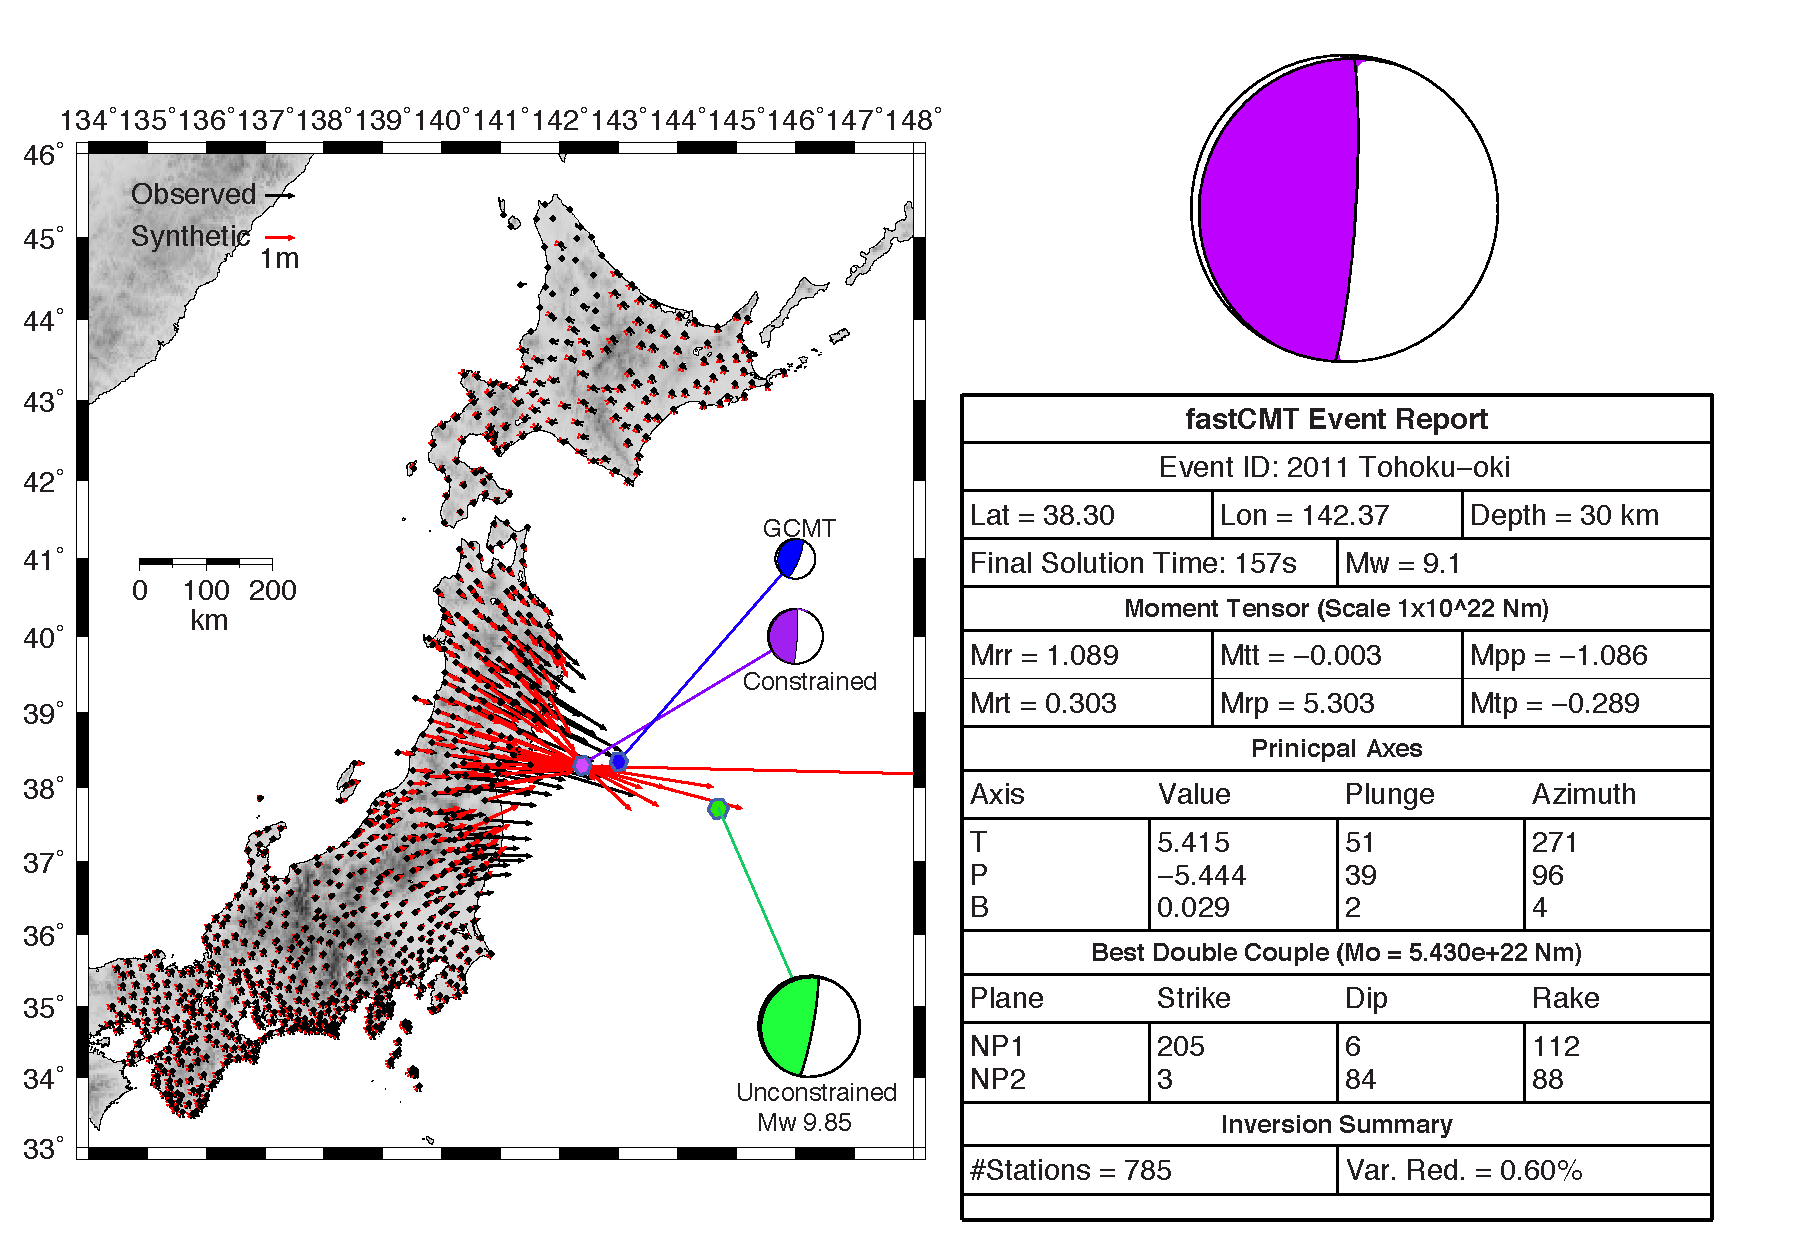
\includegraphics[width=0.99\linewidth]{./figures/ch3/tohoku_fail.pdf}
    \caption[Tohoku-oki point source inversion]{Result of the point source \textit{fast}CMT method applied to the Mw 9.0 Tohoku-oki event. The green moment tensor labeled ``unconstrained'' is the result of the grid search. The purple is the result of containing the inversion to the USGS epicenter and blue is the GCMT result. The summary table is for the inversion constrained to the USGS epicenter. Note the low variance reduction of 0.6\% in spite of the apparently good inversion parameters.}
  \label{fig_tohoku_fail}
\end{figure}

\subsection{The Finite Extent CMT Approach}

To account for source finiteness we extend the \textit{fast}CMT algorithm to a linear geometry by superposition of point sources. This is straightforward because static deformation modeling has no temporal dependence. We invert for several moment tensors at predefined points along the line source, and perform a grid search for the proper line azimuth and spatial location. For the Tohoku-oki case we assume that the Green's functions are pre-determined at inversion nodes on a 0.1$^\circ$ by 0.1$^\circ$ by 2km in depth grid to cover all of Japan with the same strategy as originally described in Section \ref{sec:pointsource}. The line source length is set to 7$^\circ$ with 30 point sources. These numbers are for the time being arbitrary and upon implementation must be tailored according to the observational goals of a particular network. We then solve the minimization problem
\begin{equation}
\label{eq_minprob}
\mathrm{min}\left\{\|\mathbf{WGm}-\mathbf{Wd}\|+\lambda\|\mathbf{Lm}\|\right\}\;,
\end{equation}
where as in Section \ref{sec:cmt} $\mathbf{m}$ is the source model, $\mathbf{G}$ the GFs, $\mathbf{W}$ the data weights determined from the variance of the pre-event noise, and $\mathbf{d}$ the coseismic offsets determined using the trailing variance technique. A major difference with the point source algorithm is that the multiple source inversion is ill-posed and requires regularization. We define $\mathbf{L}$ the smoothness matrix and $\lambda$ the smoothing parameter. The inversion scheme is, again, L1-norm minimizing with first order Tikhonov smoothing for the five deviatoric MT components. This regularization is applied to each of the 5 components of the MT with regards to the same component of the neighboring MTs along the line direction. Thus sharp variations in a particular component of the MT between neighboring point sources are penalized.

To determine the line location and azimuth we invert for multiple combinations of line geometries by varying the center of the line source, its azimuth and depth. The line source geometry that minimizes misfit in the L1 sense is the best solution. Because this inversion is computationally simple we can perform thousands of such inversions without a large computational overhead and without any assumptions required about the geometry of the source. The smoothing parameter $\lambda$ determines the roughness of the model \citep{hansen2010} and thus controls the complexity of the inversion results. It is critical to have an objective way of determining it so that no user interaction is required during an event. For this purpose we compute the tradeoff curves of data misfit $\|\mathbf{WGM}-\mathbf{Wd}\|$ versus model semi-norm $\|\mathbf{Lm}\|$ (L-curves) for a range of values of $\lambda$ (Figure \ref{fig_lcurves}a) and their optimal corners from their point of maximum curvature \citep{hansen2007,hansen2010} for all possible source geometries. We then compute the probability density function (pdf) of all values (Figure \ref{fig_lcurves}b) of $\lambda$ using the non-parametric kernel smoothing density estimate \citep{bowman1997}. We select the mode of the resulting pdf as the preferred smoothing parameter $\lambda^*$. Then, we compare the misfit of all inversions at the $\lambda^*$ optimum smoothing level and, as in the point source \textit{fast}CMT method, select the one with the smallest misfit. 

\begin{figure}[!htb] 
  \centering
  \includegraphics[width=0.85\linewidth]{./figures/ch3/lcurves.pdf}
    \caption[L-curve corner selection criterion]{(a) 3800 L-curves for line source \textit{fast}CMT inversions performed at different locations and with different orientations. Orange crosses depict the corners of each curve computed from the maximum curvature. (b) Probability density function of the smoothing parameter that corresponds to the L-curve corners. The optimum smoothing parameter $\lambda^*$ is selected from the mode of the pdf.}
  \label{fig_lcurves}
\end{figure}

The final inversion yields a variance reduction of 84\% with the GPS data alone and a slight improvement to 86\% with the seismogeodetic displacement data. We contend this marginal improvement is in part due to the one dimensional nature of the line source which does not account for along dip variations in moment release. As mentioned earlier the Kalman filter's most notable contribution to static modeling is that it better constraints the vertical offset. Later, when we discuss slip inversions we will show better control of the vertical yields improved resolution in the along dip direction. Since we have no such direction in the line source there is little improvment with the seismogeodetic derived coseismic offsets. Next, we compute the weighted average of all individual moment tensors over that line source based on their moment and place the average moment tensor at the location of mean moment release to obtain a single CMT estimate, shown in Figure \ref{fig_tohoku_slip_cmt}. This implementation of the expanded \textit{fast}CMT is unique in that no a priori information is required on the fault geometry or that the source is confined to the slab. The process is computationally simple and automatable. For this earthquake we obtain a magnitude of 9.0, average strike, dip, and rake of 204$^\circ$, 30$^\circ$, and 95$^\circ$ respectively, with a source extent of 340 km along strike. A single line inversion takes ~0.4s on a single 2.5GHz processor so the number of line sources computed in this process must be determined based on computational resources available. Also in Figure \ref{fig_tohoku_slip_cmt} is a static slip inversion obtained from inverting the seismogeodetic data, the details of this will be discussed further on, but note that the moment release of the line source bounds the main asperity in the slip inversion.

\begin{figure}[!htb] 
  \centering
  \includegraphics[width=0.65\linewidth]{./figures/ch3/tohoku_slip_cmt.pdf}
    \caption[Tohoku-oki finite extent CMT and slip inversion]{\textit{fast}CMT and slip inversion results. Green circles are the point sources superimposed to compute the line source of CMT solutions, the final averaged solution shown labeled as fastCMT, and the Global CMT solution (GCMT) shown for comparison. The inset shows the moment release from the line source as a function of distance along fault. Shown along the fault interface with 10 km depth contours from the Slab 1.0 model \citep{hayes2012} is the result of the slip inversion; the blue lines represent the direction of slip. The triangles indicate the locations of all the GPS/accelerometer stations used for computing the slip inversion. The large triangles represent the fixed GPS station (0848, red).}
  \label{fig_tohoku_slip_cmt}
\end{figure}

The finite extent moment tensor solution can be applied to smaller earthquakes, not just to the very large like the Tohoku-oki event. Consider the case of the M7.2 El Mayor-Cucapah event, we employ the same data as was used in the point source inversion and compute the line source solution, Figure \ref{fig_elmay_mt}, shows the result. We've left the line source extent parameters the same as for the Tohoku-oki case, a 0.1$^\circ$ by 0.1$^\circ$ grid of GFs is computed surrounding the event with a 2km depth interval from 0 to 30km. The line source length is set once again to 7$^\circ$ with 30 point sources. The grid search result for the best fitting line is at 4km depth and its azimuth is close to the fault plane used by \citet{Crowell2012} for a static slip inversion, which is obtained from the aftershock cloud. Note the moment release of the line source solution brackets the slip ivenrsion from \citet{Crowell2012}. This illustrates that the \textit{fast}CMT algorithm is useful, whether in its point source or line source mode for events at least between magnitudes 7 and 9.

\begin{figure}[!htb] 
  \centering
  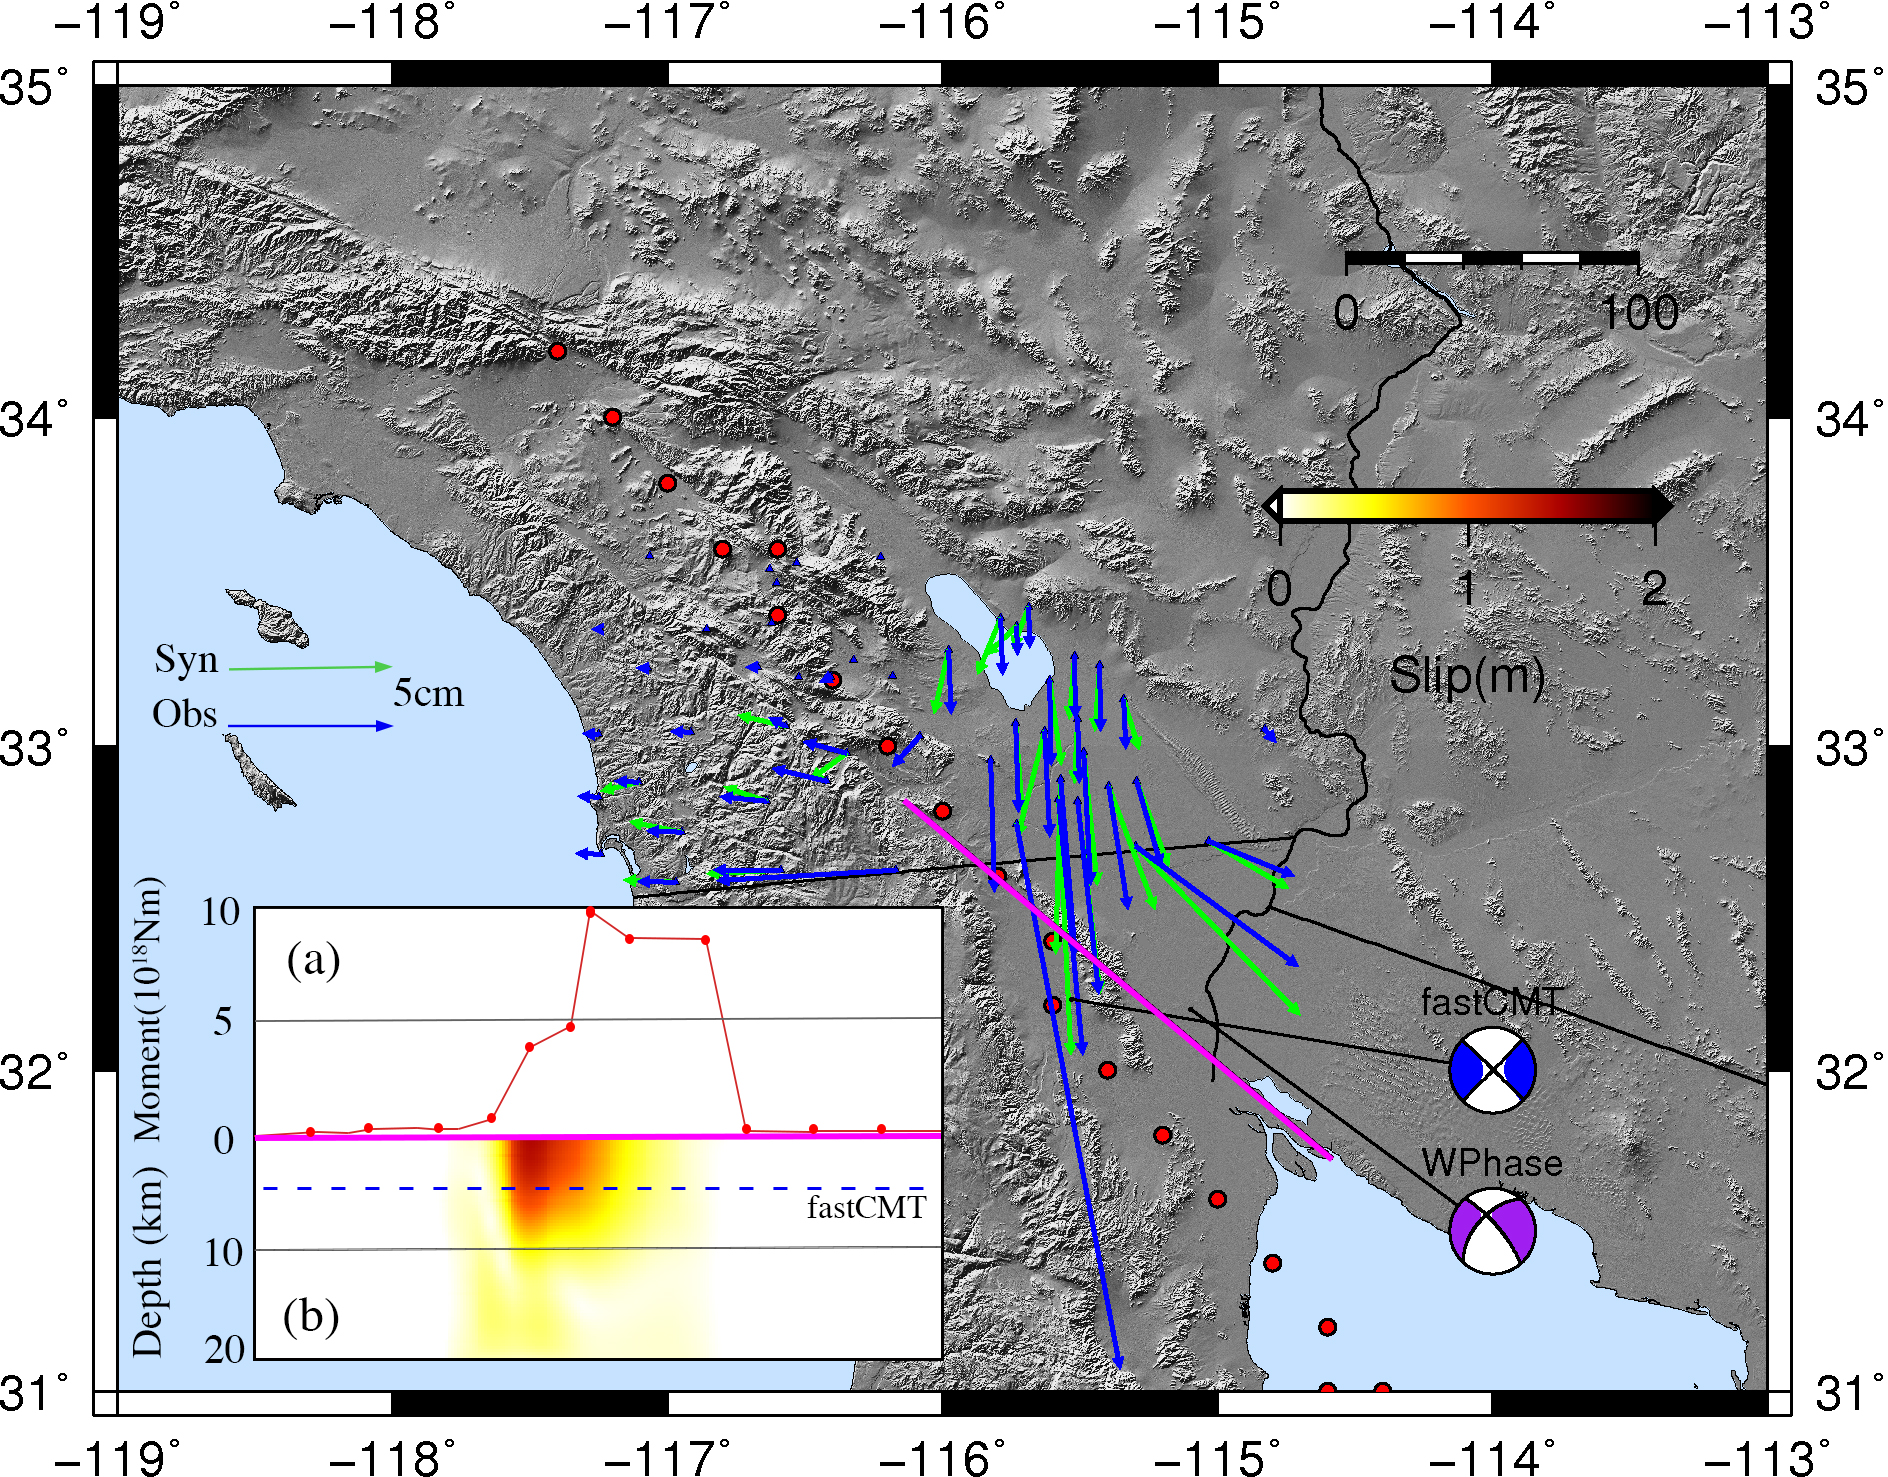
\includegraphics[width=0.9\linewidth]{./figures/ch3/elmayMT.jpg}
    \caption[El Mayor-Cucapah finite extent CMT and slip ivnersion]{\textit{fast}CMT and slip inversion results. Red circles are the point sources superimposed to compute the line source of CMT solutions, the final averaged solution shown labeled as fastCMT, and the USGS W-Phase solution shown for comparison. The inset (a) shows the moment release from the line source as a function of distance along fault. (b) is the slip inversion from \citet{Crowell2012} which uses the same GPS data as the moment tensor inversion. The blue dashed line shows tend depth of the \textit{fast}CMT solution}
  \label{fig_elmay_mt}
\end{figure}

\section{Static Slip Inversions}

After determining the style off faulting and the approximate geographical extent of rupture the next logical step is to perform a slip inversion with the static field data. We will not discuss this in great depth because it was thoroughly discussed in a previous dissertation \citep{crowell2013thesis}. However, we have expanded on the automatic determination of the regularization parameter and analyzed the benefits of inverting with the seismogeodetic as opposed to just the GPS data,  a brief discussion follows.

Modifications to the work of \citet{crowell2013thesis} are best illustrated by analyzing the Tohoku-oki case. For a real-time implementable system one cannot simply assume that all large ruptures occur on the megathrust. Several recent event events illustrate this. The Mw 8.6 event in the Wharton Basin off Sumatra, Indonesia, on 11 April 2012 \citep{satriano2012} was a predominantly a strike-slip event on the oceanic plate whose rupture arrested very close to the trench. The Mw 8.1 Samoa event on 29 September 2009 was a normal faulting, outer-rise type event that produced a sizeable tsunami with 189 fatalities \citep{okal2010}. Furthermore, the 2012-2013 Haida Gwaii and Craig events where a thrust and strike-slip earthquake a few months apart \citep{lay2013} on the same oblique plate boundary. Subduction zones can and do produce many types of earthquakes. Thus it is critical to analyze the CMT information before computation of a slip inversion.

In the Tohoku case after receiving information on the style of faulting and the centroid from the \textit{fast}CMT analysis and determining that it is a thrust event close to the slab, we invert for static slip using the same coseismic offsets and data weights. For the static slip inversion, we first locate the closest fault segment from the Slab1.0 model \citep{hayes2012} to the line source. The fault is then subdivided into $25\times25$km segments. GFs are then computed for every subfault-station pair. We use Laplacian smoothness as $\mathbf{L}$ with the traditional $(1,1,-4,1,1)$ finite difference stencil in Equation \ref{eq_minprob}.  As in the \textit{fast}CMT solution, an optimal smoothing parameter $\lambda^* $ is determined from the maximum curvature of the L-curve (Figure \ref{fig_tohoku_lcurve}). We constrain the edges and bottom of the fault to zero to avoid non-physical slip distributions in the model (i.e., step-function motion at the edges). The fault segments at the trench are left freely slipping to accommodate shallow slip. The inverse problem is solved by minimizing the L2-norm in Equation \ref{eq_minprob}. This solution takes several seconds to complete after the extended CMT solution becomes available.

\begin{figure}[!htb] 
  \centering
  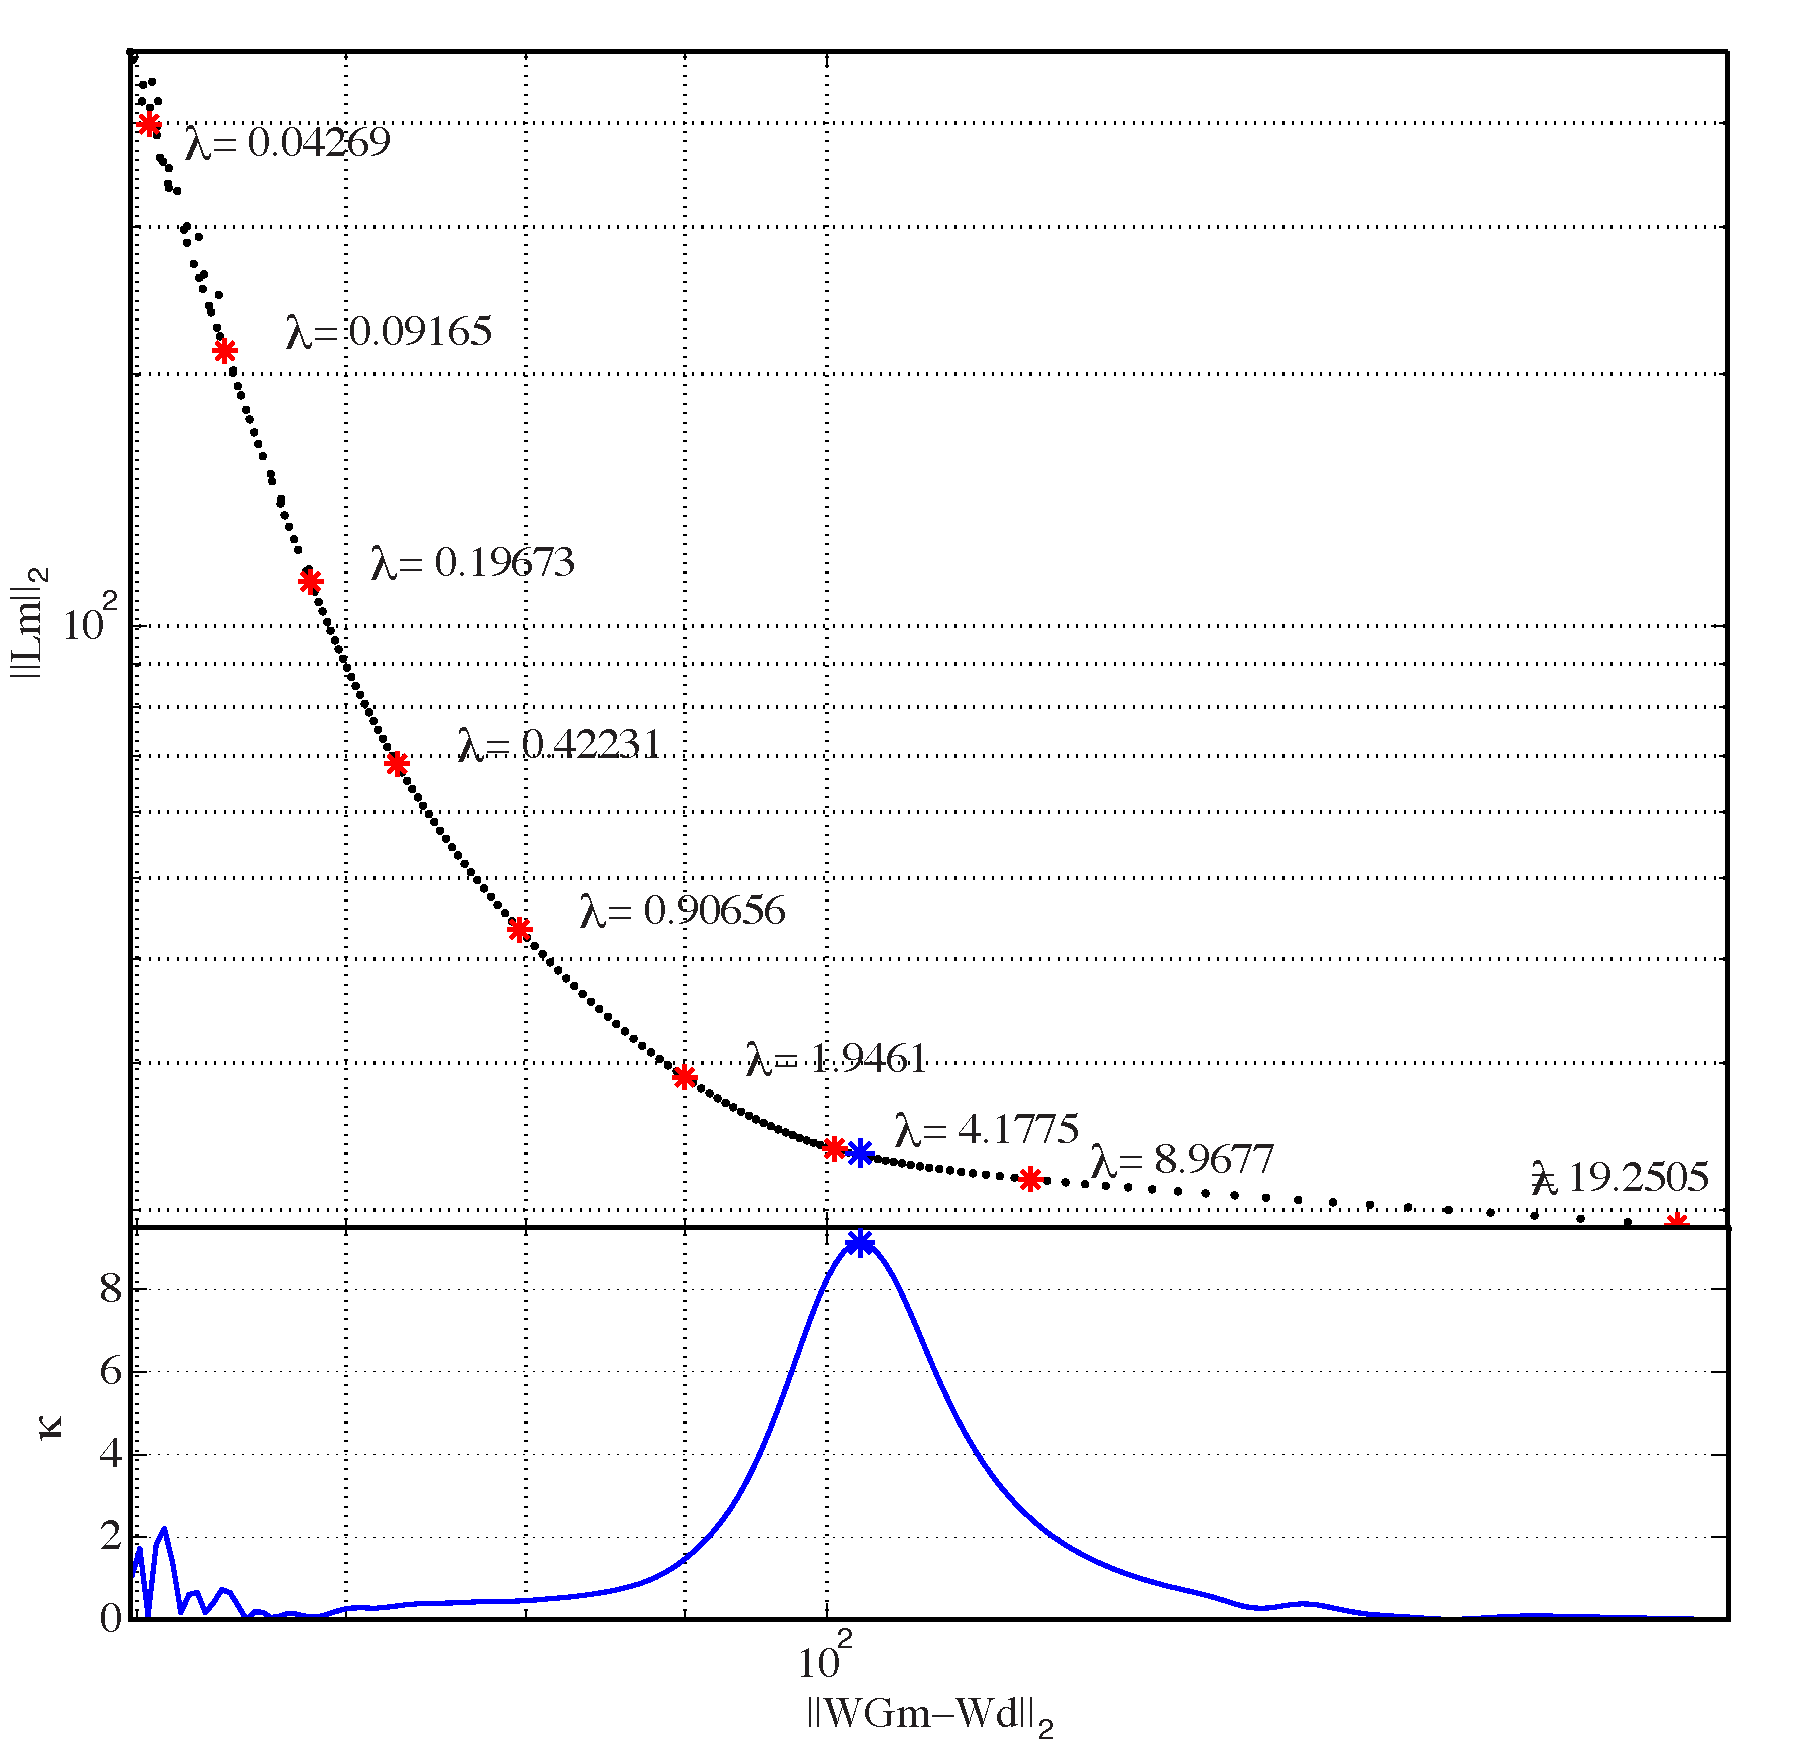
\includegraphics[width=0.8\linewidth]{./figures/ch3/tohoku_lcurve.pdf}
    \caption[Tohoku-oki slip inversion L-curve]{L-curve for the slip inversion plotting the model seminorm $\|\mathbf{Lm}\|_2$ versus model misfit $\|\mathbf{WGm}-\mathbf{Wd}\|_2$ with solutions at selected values of the smoothing parameter $\lambda$ plotted as red stars. Also plotted is the curvature $\kappa$ of the L-curve, the optimum smoothing parameter $\lambda^*$ is selected as the value that corresponds to the maximum curvature (blue star).}
  \label{fig_tohoku_lcurve}
\end{figure}

Our model indicates a moment magnitude of 8.9, a slip patch that is roughly 340km along-strike and 155km along-dip, and maximum slip of 27m located near the center of the \textit{fast}CMT location at 14km depth. We know now that in order to fit seafloor geodetic measurements of displacement outboard of the trench that were surveyed up to a month after the earthquake, static slip inversions with a maximum slip closer to 50m \citep{sato2011} are necessary. However, seafloor geodetic measurements are currently not available in real time and would include some amount of postseismic deformation, so our model is indicative of a realistic real-time scenario using just land-based seismogeodetic data. In Chapter 5 we'll show that using cabled seafloor pressure gauge data and seismogeodetic offsets one can produce maximum slip of 50m. It is of course, possible to obtain models with higher amounts of slip by reducing the smoothing constraint, but these are not selected under the automated operator-independent L-curve criterion we present here. The moment release from the line source \textit{fast}CMT overlain upon the slip distribution in Figure \ref{fig_tohoku_slip_cmt} shows the slip distribution is bounded by the line source moment release along strike, indicating that both methods independently agree on the spatial extent of slip. The dip of the \textit{fast}CMT solution (30$^\circ$) is larger than the average dip for the slab in the region ($\sim15^\circ$), possibly because of the unmolded along-dip dimension. This demonstrates the importance of having both the slip inversion and \textit{fast}CMT to independently validate results and guide response. We also perform the slip inversion and \textit{fast}CMT using just the GPS data for the same stations to investigate improvements with seismogeodetic data. We find that vertical bias (median difference of 18mm) in the GPS-only slip inversion solution leads to far more deep slip and significantly less shallow slip than the seismogeodetic solution (Figure \ref{fig_tohoku_depthbias}) and a 4$^\circ$ difference in the average rake (84$^\circ$ for combined data and 88$^\circ$ for GPS-only data). This is due to the improved precision in the vertical offset estimates from seismogeodetic data and greater weights assigned to the improved vertical channel in the inversion, yielding better along-dip model resolution.

\begin{figure}[!htb] 
  \centering
  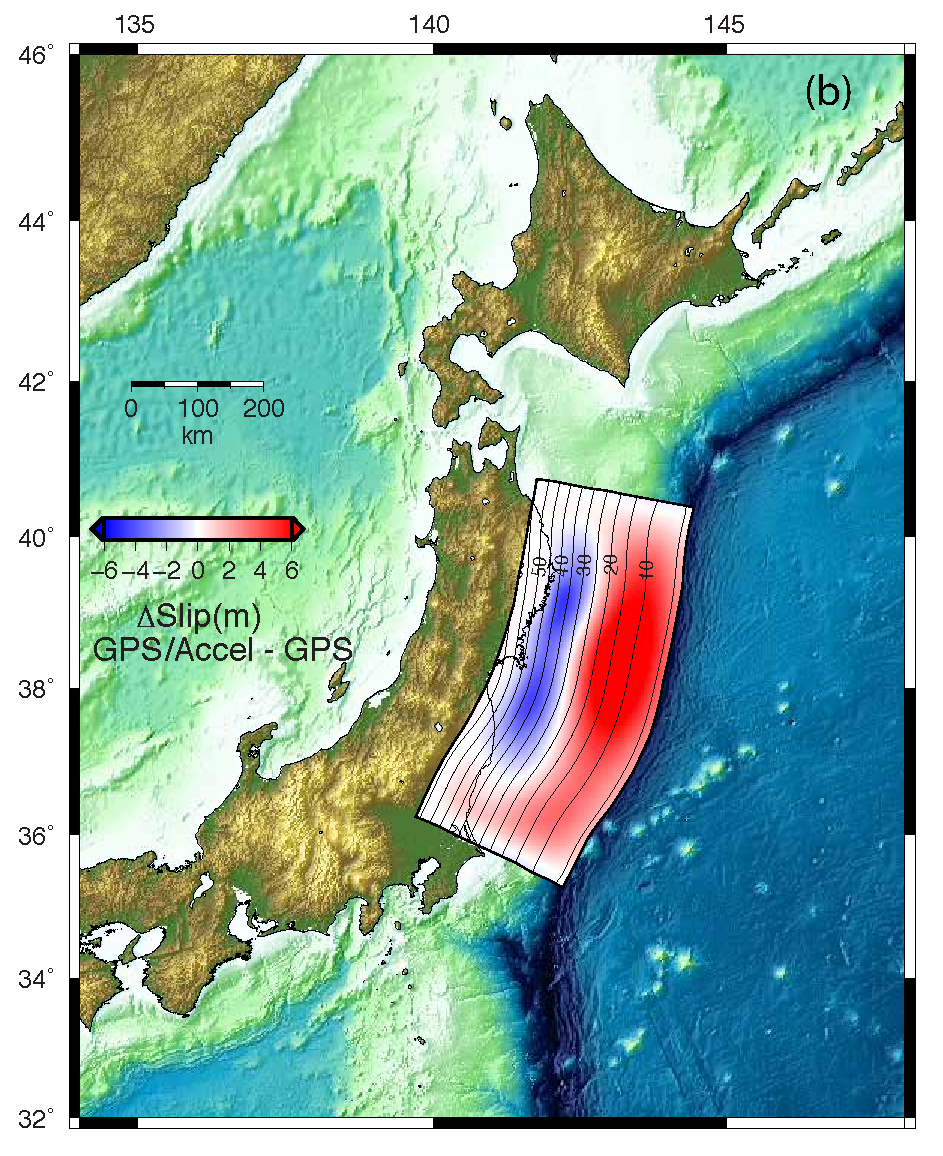
\includegraphics[width=0.7\linewidth]{./figures/ch3/tohoku_depthbias.pdf}
    \caption[Tohoku-oki slip inversion depth biases]{Difference between slip inversions computed using the improved precision GPS/accelerometer displacements vs. the inversion carried out using the GPS-only derived displacements. Red indicates more slip with the seismogeodetic solution and blue indicates more slip with the GPS-only solution.}
  \label{fig_tohoku_depthbias}
\end{figure}

\subsection{Timeline of Event Analysis}

Based upon the aforementioned approach, we propose the following timeline of effective warnings for an augmented seismogeodetic earthquake early warning and rapid response system. Based on our experience with operational real-time networks in Western U.S. that employ a variety of communication links, raw data are continuously collected from the stations within a fraction of a second \citep{Bock2004}, and seismogeodetic displacements and velocities are estimated continuously with a latency of about 1s. The origin time and hypocenter can be calculated from the first detections of \textit{P} waves at a subset of seismic or seismogeodetic instruments using existing methodologies. For the Tohoku-oki data set, the time of arrival of \textit{P} waves at the first stations is 24 seconds after earthquake initiation. Line-source CMT solutions are initiated based on the displacements exceeding a threshold (Section \ref{sec:cmt}) and thus independently confirm, rather than rely on, the seismic network hypocenter. The line-source CMT solutions computed from the coseismic offsets by 157s after rupture initiation determine an initial magnitude, location and style of faulting, as well as provide rough constraints on the lateral extent of moment release; the duration of the Tohoku-oki earthquake rupture was $\sim180s$ \citep{simons2011}. From the line source CMT solutions, we are able to determine an appropriate section of fault to perform a heterogeneous static slip inversion. The slip inversion can run immediately after the CMT computation, so a full heterogeneous slip distribution is determined within seconds of the CMT solution. Model resolution in the along-dip direction is significantly improved with seismogeodetic offset estimates; this is critical for accurate tsunami modeling since it directly impacts vertical seafloor deformation estimates. After the slip inversion, obvious next steps would include ingestion into ShakeMap, PAGER maps, tsunami forward modeling to ascertain near-field inundation models \citep{Ohta2012}, kinematic slip inversions, and further analysis to capture aftershocks and postseismic deformation.

This is all assuming satisfactory solution of an inverse problem. In any such problem the critical determination of the smoothing parameter typically requires operator decision-making. Here we have presented and implemented a simple algorithm that adds minimal computational overhead to guide the determination of this critical parameter that requires no human interaction and produces actionable models. In summary, the methods proposed here are computationally efficient and are able to be implemented in real time, with minimal prior assumptions.

\section{Acknowledgments}

For sections 3.1.1 to 3.1.4 The work was funded by NASA/AIST Grant No. NNX09AI67G and is published in \textbf{Melgar, D., Bock, Y., and Crowell, B.W., ``Real-Time Centroid Moment Tensor Determination for Large Earthquakes from Local and Regional Displacement Records'', \emph{Geophys. J. Int.}, 188(2), 2012.}. For Sections 3.1.5-3.1.6 and 3.2 we would like to thank NIED for access to K-NET and KiK-net accelerometer data and GSI for GEONET GPS data. Suggestions provided by Rob Clayton, Sharon Kedar, and Tim Melbourne are appreciated. The work was funded by NASA Grants NNX09AI67G, NNX12AK24G, and NNX12AN55H and SCEC award 12083. The work is published in \textbf{Melgar, D., Crowell, B.W., Bock, Y., and Haase, J.S, ``Rapid modeling of the 2011 Mw 9.0 Tohoku-oki earthquake with seismogeodesy'', \emph{Geophys. Res. Lett}, 40(12), 2013}



%\appendix
%\chapter{Final notes}
%  Remove me in case of abdominal pain.

